\باب{خطی الجبرا: امتیازی قدر مسائل قالب}
امتیازی قدر مسائل درج ذیل سمتی مساوات پر مبنی ہیں جہاں \عددی{\bM{A}} چکور قالب، \عددی{\bM{x}} نا معلوم سمتیہ اور \عددی{\lambda} نا معلوم غیر سمتیہ ہے۔
\begin{align}\label{مساوات_امتیازی_مسئلہ_الف}
\bM{A}\bM{x}=\lambda \bM{x}
\end{align}
امتیازی قدر مسائل میں ہمیں وہ \عددی{\lambda} اور \عددی{\bM{x}} درکار ہیں جو درج بالا مساوات پر پورا اترتے ہوں۔ \عددی{\lambda} کی ہر قیمت کے لئے 
 \عددی{\bM{x}=\bM{0}} مساوات \حوالہ{مساوات_امتیازی_مسئلہ_الف} کا غیر اہم صفر حل ہے۔ ہم اس غیر اہم صفر حل میں دلچسپی نہیں رکھتے ہیں لہٰذا ہم غیر صفر حل \عددی{\bM{x} \ne \bM{0}} جاننا چاہیں گے۔

\عددی{\lambda} کی وہ قیمتیں جو مساوات \حوالہ{مساوات_امتیازی_مسئلہ_الف} پر پورا اترتے ہیں \عددی{\bM{A}} کے \اصطلاح{امتیازی اقدار}\فرہنگ{امتیازی اقدار} یا \اصطلاح{امتیازی اقدار}\فرہنگ{امتیازی اقدار}\حاشیہب{eigenvalues}\فرہنگ{eigenvalues} کہلاتے ہیں اور وہ \عددی{\bM{x}} جو مساوات \حوالہ{مساوات_امتیازی_مسئلہ_الف} پر پورا اترتے ہیں \عددی{\bM{A}} کے \اصطلاح{امتیازی سمتیات}\فرہنگ{امتیازی!سمتیات} یا \اصطلاح{امتیازی تفاعل}\فرہنگ{امتیازی!تفاعل}\حاشیہب{eigenfunctions}\فرہنگ{eigenfunctions} کہلاتے ہیں۔

اس معصوم نظر آنے والا سمتی مساوات کے اندر حیران کن تفصیل چھپی ہے۔امتیازی قدر مسائل انجینئری، طبیعیات، ریاضی، حیاتیات، ماحولیاتی سائنس، شہری منصوبہ بندی،  معاشیات، نفسیات اور دیگر شعبوں میں عموماً درپیش آتے ہیں۔آپ کو یقیناً ان سے زندگی میں واسطہ پڑے گا۔

%=============
\حصہ{امتیازی قدر مسائل قالب۔ امتیازی اقدار اور امتیازی سمتیات کا حصول}\شناخت{حصہ_امتیازی_اقدار_اور_سمتیات}
درج ذیل پر غور کریں جہاں غیر صفر سمتیہ اور چکور قالب کے ضرب دکھائے گئے ہیں۔
\begin{align}\label{مساوات_امتیازی_پہلی_مثال}
\begin{bmatrix}6&3\\4&7  \end{bmatrix}\begin{bmatrix} 5\\1 \end{bmatrix}=\begin{bmatrix}33\\27  \end{bmatrix},\quad \begin{bmatrix}6&3\\4&7  \end{bmatrix}\begin{bmatrix} 3\\4 \end{bmatrix}=\begin{bmatrix}30\\40  \end{bmatrix}
\end{align} 
بائیں ہاتھ کی ضرب میں ہمیں مکمل طور پر نیا سمتیہ حاصل ہوتا ہے جس کی لمبائی اور سمت ابتدائی سمتیہ کی لمبائی اور سمت  سے مختلف ہیں۔عموماً  سمتیہ کو چکور قالب سے ضرب دینے  سے مکمل طور پر مختلف سمتیہ حاصل ہوتا ہے۔دائیں ہاتھ کی ضرب میں حاصل سمتیہ کو درج ذیل لکھا جا سکتا ہے 
\begin{align*}
\begin{bmatrix}30\\40  \end{bmatrix}=10\begin{bmatrix}3\\4  \end{bmatrix}
\end{align*}
یعنی حاصل سمتیہ اور ابتدائی سمتیہ کی سمتیں ایک جیسی ہیں جبکہ حاصل سمتیہ کی لمبائی ابتدائی سمتیہ کی لمبائی کے دس گنّا ہے جس کو \عددی{\lambda=10} لکھا جائے گا۔چکور قالب \عددی{\bM{A}} کے لحاض سے  ایسے \عددی{\lambda} اور غیر صفر سمتیات کا حصول اس باب کا مرکزی مضمون ہے۔  

آئیں درج بالا مشاہدے کو دستوری شکل دیں۔فرض کریں کہ \عددی{\bM{A}=[a_{jk}]} غیر صفر \عددی{n\times n} جسامت کا چکور قالب ہے۔اب درج ذیل سمتی مساوات پر غور کریں۔
\begin{align}\label{مساوات_امتیازی_مسئلہ_ب}
\bM{A}\bM{x}=\lambda \bM{x}
\end{align}
ان \عددی{\lambda} اور غیر صفر \عددی{\bM{x}} کے حصول کے مسئلے کو، جو مساوات \حوالہ{مساوات_امتیازی_مسئلہ_ب} پر پورا اترے ہوں،  \اصطلاح{امتیازی قدر مسئلہ}\فرہنگ{امتیازی قدر مسئلہ}\فرہنگ{مسئلہ!امتیازی قدر} کہتے ہیں۔

یہاں توجہ دیں کہ \عددی{\bM{A}} دیا گیا چکور قالب ہے جبکہ \عددی{\lambda} نا معلوم غیر سمتیہ اور \عددی{\bM{x}} نا معلوم سمتیہ ہے۔ہم وہ \عددی{\lambda} اور \عددی{\bM{x}} حاصل کرنا چاہتے ہیں جو مساوات \حوالہ{مساوات_امتیازی_مسئلہ_ب} پر پورا اترتے ہوں۔ جیومیٹریائی طور پر ہم وہ سمتیات \عددی{\bM{x}} حاصل کرنا چاہتے ہیں جنہیں \عددی{\bM{A}} سے ضرب دینا ایسا ہی ہے جیسے ان سمتیوں کو غیر سمتی \عددی{\lambda} سے ضرب دیا جائے یعنی کہ \عددی{\bM{A}\bM{x}} اور \عددی{\bM{x}} راست تناسب ہوں۔یوں مثبت \عددی{\lambda} کی صورت میں ابتدائی اور حاصل سمتیات کی سمتیں ایک جیسی ہوں گی جبکہ منفی \عددی{\lambda} کی صورت میں ان کی سمتیں آپس میں الٹ ہوں گی۔ (باب کی شروع میں سادہ مثال سے اس کی وضاحت کی گئی ہے۔)

 \عددی{\lambda} کی وہ مخصوص قیمت جس کے لئے مساوات \حوالہ{مساوات_امتیازی_مسئلہ_ب} کے غیر صفر \عددی{\bM{x}\ne \bM{0}} حل موجود ہوں  \عددی{\bM{A}} کی \اصطلاح{امتیازی قدر}\فرہنگ{امتیازی!قدر}\حاشیہب{eigenvalue}\فرہنگ{eigenvalue} کہلاتی ہے اور مطابقتی سمتیات \عددی{\bM{x}}،  اس \عددی{\lambda} کے لحاض سے قالب \عددی{\bM{A}} کے  \اصطلاح{امتیازی سمتیات}\فرہنگ{امتیازی!سمتیات}\حاشیہب{eigenvectors}\فرہنگ{eigenvectors} یا \اصطلاح{امتیازی سمتیات}\فرہنگ{امتیازی!سمتیات}\حاشیہب{characteristic vectors}\فرہنگ{characteristic vectors} کہلاتے ہیں۔\عددی{\bM{A}} کے تمام امتیازی اقدار کو \عددی{\bM{A}} کا \اصطلاح{طیف}\فرہنگ{طیف}\حاشیہب{spectrum}\فرہنگ{spectrum} کہتے ہیں۔طیف میں کم سے کم ایک عدد امتیازی قدر اور زیادہ سے زیادہ \عددی{n} مختلف امتیازی اقدار ہو سکتے ہیں۔ امتیازی اقدار کی سب سے  زیادہ حتمی قیمت کو \عددی{\bM{A}} کا \اصطلاح{رداس طیف}\فرہنگ{رداس!طیف}\فرہنگ{طیف!رداس}\حاشیہب{spectral radius}\فرہنگ{spectral radius} کہتے ہیں۔

امتیازی قدر مسئلے کا حل چند مثالوں کی مدد سے سیکھتے ہیں۔
%=================
\ابتدا{مثال}\شناخت{مثال_امتیازی_اقدار_الف}\quad امتیازی اقدار اور امتیازی سمتیات کا حصول\\
درج ذیل قالب کے امتیازی اقدار اور امتیازی سمتیات قدم بہ قدم دریافت کرتے ہیں۔
\begin{align*}
\bM{A}=\begin{bmatrix*}[r] -5&2\\2&-2 \end{bmatrix*}
\end{align*}
پہلے امتیازی اقدار دریافت کیے جاتے ہیں۔مساوات \حوالہ{مساوات_امتیازی_مسئلہ_ب} درج ذیل ہو گا۔
\begin{gather*}
\bM{A}\bM{x}=\begin{bmatrix*}[r] -5&2\\2&-2 \end{bmatrix*}\begin{bmatrix} x_1\\x_2 \end{bmatrix}=\lambda \begin{bmatrix} x_1\\x_2 \end{bmatrix};\quad \implies \quad \begin{aligned}-5x_1+2x_2&=\lambda x_1\\ 2x_1-2x_2&=\lambda x_2\end{aligned}
\end{gather*}
تمام اجزاء کو ایک طرف منتقل کرتے ہوئے
\begin{gather}
\begin{aligned}\label{مساوات_امتیازی_مثال_الف}
(-5-\lambda)x_1+2x_2&=0\\
2x_2+(-2-\lambda)x_2&=0
\end{aligned}
\end{gather}
قالبی صورت میں لکھتے ہیں۔
\begin{align*}
(\bM{A}-\lambda \bM{I})\bM{x}=\bM{0}
\end{align*}
مسئلہ \حوالہ{مساوات_الجبرا_مسئلہ_کریمر_عمومی} کے تحت اس متجانس نظام کا غیر صفر اہم حل \عددی{\bM{x} \ne \bM{0}} (قالب \عددی{\bM{A}} کا امتیازی سمتیہ جس کی ہمیں تلاش ہے)  اس صورت ممکن ہو گا جب عددی سر قالب کا مقطع صفر کے برابر ہو گا۔
\begin{align*}
D(\lambda)=\begin{vmatrix} -5-\lambda& 2\\ 2 & -2-\lambda \end{vmatrix}=(-5-\lambda)(-2-\lambda)-4=\lambda^2+7\lambda+6=0
\end{align*}
ہم \عددی{D(\lambda)} کو \عددی{\bM{A}} کی \اصطلاح{امتیازی مقطع} جبکہ اس کی پھیلی  ہوئی صورت کو \اصطلاح{امتیازی کثیر رکنی} اور \عددی{D(\lambda)=0} کو \اصطلاح{امتیازی مساوات} کہتے ہیں۔اس دو درجی الجبرائی مساوات کے حل \عددی{\lambda_1=-1} اور \عددی{\lambda_2=-6} ہیں جو \عددی{\bM{A}} کے امتیازی اقدار ہیں۔

\عددی{\lambda_1=-1} کا مطابقتی امتیازی سمتیہ مساوات \حوالہ{مساوات_امتیازی_مثال_الف} میں \عددی{\lambda=\lambda_1=-1} پر کرتے ہوئے حاصل کرتے ہیں۔
\begin{gather*}
\begin{aligned}
[-5-(-1)]x_1+2x_2&=0\\
2x_2+[-2-(-1)]x_2&=0
\end{aligned}\quad \implies \quad \begin{aligned} -4x_1+2x_2&=0\\2x_2-x_2&=0 \end{aligned}
\end{gather*}
ان میں سے کسی بھی مساوات کو حل کرتے ہوئے  \عددی{x_2=2x_1} ملتا ہے جس کو استعمال کرتے ہوئے متعدد متوازی امتیازی سمتیات حاصل کیے جا سکتے ہیں۔یوں \عددی{x_1} (یا \عددی{x_2}) کی کوئی بھی قیمت چن کر\عددی{x_2} (\عددی{x_1}) حاصل کرتے ہوئے امتیازی سمتیہ حاصل ہو گا۔ہم \عددی{x_1=1} چن کر \عددی{x_2=2} حاصل کرتے ہیں اور یوں \عددی{\bM{x}_1=[1 \quad 2]^T} ہو گا۔اس جواب کی تصدیق کرتے ہیں۔
\begin{align*}
\bM{A}\bM{x}_1=\begin{bmatrix*}[r] -5&2\\2&-2 \end{bmatrix*}\begin{vmatrix} 1\\2 \end{vmatrix}=\begin{bmatrix}-1\\-2  \end{bmatrix}=(-1)\bM{x}_1=\lambda_1\bM{x}_1
\end{align*}
\عددی{\lambda_2=-6} کا مطابقتی امتیازی سمتیہ مساوات \حوالہ{مساوات_امتیازی_مثال_الف} میں \عددی{\lambda=\lambda_1=-6} پر کرتے ہوئے حاصل کرتے ہیں۔
\begin{gather*}
\begin{aligned}
[-5-(-6)]x_1+2x_2&=0\\
2x_2+[-2-(-6)]x_2&=0
\end{aligned}\quad \implies \quad \begin{aligned} x_1+2x_2&=0\\2x_2+4x_2&=0 \end{aligned}
\end{gather*}
ان میں سے کسی بھی مساوات کو حل کرتے ہوئے \عددی{x_2=-\tfrac{1}{2}x_1} ملتا ہے۔یوں \عددی{x_1=2} چنتے ہوئے  \عددی{x_2=-1} ملتا ہے لہٰذا \عددی{\lambda_2=-6} کا مطابقتی امتیازی سمتیہ \عددی{\bM{x}_2=[2\quad -1]^T} ہو گا۔اس کی تصدیق کرتے ہیں۔
\begin{align*}
\bM{A}\bM{x}_2=\begin{bmatrix*}[r] -5&2\\2&-2 \end{bmatrix*}\begin{vmatrix} 2\\-1 \end{vmatrix}=\begin{bmatrix}-12\\6  \end{bmatrix}=(-6)\bM{x}_2=\lambda_2\bM{x}_2
\end{align*}
آپ حصہ \حوالہ{حصہ_امتیازی_اقدار_اور_سمتیات} کے آغاز میں مساوات \حوالہ{مساوات_امتیازی_پہلی_مثال} میں دیے گئے مثال کو حل کرتے ہوئے  امتیازی اقدار \عددی{10}، \عددی{3} اور  مطابقتی امتیازی سمتیات \عددی{[3\quad 4]^T}، \عددی{[-1\quad 1 ]^T} حاصل کریں۔
\انتہا{مثال}
%=====================

درج بالا مثال میں استعمال کی گئی ترکیب کی عمومی صورت پیش کرتے ہیں۔ مساوات \حوالہ{مساوات_امتیازی_مسئلہ_ب} کو اجزاء کی صورت میں درج ذیل لکھا جا سکتا ہے۔
\begin{gather}
\begin{aligned}\label{مساوات_امتیازی_متجانس_نظام_الف}
a_{11}x_1+\cdots +a_{1n}x_n&=\lambda x_1\\
a_{21}x_1+\cdots +a_{2n}x_n&=\lambda x_2\\
\vdots&\\
a_{n1}x_1+\cdots +a_{nn}x_n&=\lambda x_n\\
\end{aligned}
\end{gather}
تمام اجزاء کو بائیں ہاتھ منتقل کرتے ہیں۔
\begin{gather}
\begin{aligned}\label{مساوات_امتیازی_متجانس_نظام_ب}
(a_{11}-\lambda)x_1+a_{12}x_2+\cdots +a_{1n}x_n&=0\\
a_{21}x_1+(a_{22}-\lambda)x_2+\cdots +a_{2n}x_n&=0\\
\vdots&\\
a_{n1}x_1+a_{n2}x_2+\cdots +(a_{nn}-\lambda)x_n&=0\\
\end{aligned}
\end{gather}
اس کو قالب کی صورت میں لکھتے ہیں۔
\begin{align}\label{مساوات_امتیازی_متجانس_نظام_پ}
(\bM{A}-\lambda \bM{I})\bM{x}=0
\end{align}
مسئلہ کریمر (مسئلہ \حوالہ{مساوات_الجبرا_مسئلہ_کریمر_عمومی}) کے تحت درج بالا متجانس نظام کا غیر صفر حل صرف اور صرف اس صورت ممکن ہو گا جب  اس کے عددی سر قالب کا مقطع صفر کے برابر ہو:
\begin{align}\label{مساوات_امتیازی_متجانس_نظام_ت}
D(\lambda)=\begin{vmatrix} a_{11}-\lambda & a_{12}&\cdots & a_{1n} \\ a_{21}& a_{22}-\lambda&\cdots & a_{2n}\\ \vdots \\ a_{n1}& a_{n2}&\cdots & a_{nn}-\lambda \end{vmatrix}=0
\end{align} 
\عددی{\bM{A}-\lambda\bM{I}} کو \عددی{\bM{A}} کا \اصطلاح{امتیازی قالب}\فرہنگ{امتیازی!قالب}\فرہنگ{قالب!امتیازی}  جبکہ \عددی{D(\lambda)}  کو \عددی{\bM{A}} کا \اصطلاح{امتیازی مقطع}\فرہنگ{امتیازی!مقطع}\فرہنگ{مقطع!امتیازی} کہتے ہیں۔ مساوات \حوالہ{مساوات_امتیازی_متجانس_نظام_ت} کو \عددی{\bM{A}} کی \اصطلاح{امتیازی مساوات}\فرہنگ{امتیازی!مساوات}\فرہنگ{مساوات!امتیازی} کہتے ہیں۔مساوات \حوالہ{مساوات_امتیازی_متجانس_نظام_ت} کو پھیلا کر \عددی{\bM{A}} کی امتیازی کثیر رکنی حاصل ہو گی۔

مساوات \حوالہ{مساوات_امتیازی_متجانس_نظام_ت} کو پھیلا کر حاصل کثیر رکنی میں \عددی{\lambda^n} بلند تر طاقت ہے لہٰذا اس سے زیادہ سے زیادہ \عددی{n} مختلف امتیازی اقدار حاصل ہو سکتے ہیں۔ 
%========================

\ابتدا{مسئلہ}\شناخت{مسئلہ_امتیازی_اقدار}\quad امتیازی اقدار\\
چکور قالب \عددی{\bM{A}} کے امتیازی اقدار \عددی{\bM{A}} کے امتیازی مساوات \حوالہ{مساوات_امتیازی_متجانس_نظام_ت} سے حاصل ہوں گے۔\\
یوں \عددی{n\times n} قالب کی کم سے کم ایک عدد امتیازی قدر اور زیادہ سے زیادہ \عددی{n} مختلف  امتیازی اقدار ہو سکتے ہیں۔
\انتہا{مسئلہ}
%=============================

\عددی{n} کی بڑی قیمت کی صورت میں امتیازی اقدار عموماً ترکیب نیوٹن یا کسی اور اعدادی ترکیب سے حاصل کئے جائیں گے۔

امتیازی اقدار پہلے حاصل کیے جاتے ہیں۔باری باری ان امتیازی قدر کو مساوات \حوالہ{مساوات_امتیازی_متجانس_نظام_ب} کے نظام میں پر کرتے ہوئے مطابقتی امتیازی سمتیہ ( گاوسی اسقاط کی مدد سے) حاصل کیا جاتا ہے۔

امتیازی سمتیات درج ذیل خصوصیات رکھتے ہیں۔
%=================

\ابتدا{مسئلہ}\شناخت{مسئلہ_امتیازی_سمتیہ_فضا}\quad امتیازی سمتیات اور امتیازی فضا\\
اگر قالب \عددی{\bM{A}} کے کسی ایک امتیازی قدر \عددی{\lambda} کے مطابقتی امتیازی سمتیات \عددی{\bM{w}} اور \عددی{\bM{x}} ہوں تب \عددی{\bM{w}+\bM{x}} (بشرطیکہ \عددی{\bM{w} \ne -\bM{x}} ہو) اور \عددی{k\bM{x}} جہاں \عددی{k\ne 0} ہے بھی اس \عددی{\lambda} کے مطابقتی بھی امتیازی سمتیات ہوں گے۔

یوں کسی ایک امتیازی قدر کے مطابقتی امتیازی سمتیات اور \عددی{\bM{0}} سمتیہ مل کر فضا بناتے ہیں جس کو اس \عددی{\lambda} کے لئے \عددی{\bM{A}} کی مطابقتی  \اصطلاح{امتیازی فضا} کہتے ہیں۔
\انتہا{مسئلہ}
%============================

\ابتدا{ثبوت}
\عددی{\bM{A}\bM{w}=\lambda \bM{w}} اور \عددی{\bM{A}\bM{x}=\lambda \bM{x}} سے مراد درج ذیل ہے
\begin{align*}
\bM{A}(\bM{w}+\bM{x})=\bM{A}\bM{w}+\bM{A}\bM{x}=\lambda \bM{w}+\lambda\bM{x}=\lambda(\bM{w}+\bM{x})
\end{align*}
اور \عددی{\bM{A}(k\bM{w})=k(\bM{A}\bM{w})=k(\lambda \bM{w})=\lambda(k\bM{w})} ہے لہٰذا \عددی{\bM{A}(k\bM{w}+l\bM{x})=\lambda(k\bM{w}+l\bM{x})} ہو گا۔
\انتہا{ثبوت}
%===============================

امتیازی سمتیہ کو معیار سے تقسیم کرتے ہوئے \اصطلاح{معیاری امتیازی سمتیہ}  یعنی \اصطلاح{اکائی امتیازی سمتیہ} حاصل کیا جا سکتا ہے۔مثلاً مثال \حوالہ{مثال_امتیازی_اقدار_الف} میں \عددی{\bM{x}_1=[1 \quad 2]^T} کی لمبائی \عددی{\norm{\bM{x}_1}=\sqrt{1^2+2^2}=\sqrt{5}} ہے جس سے معیاری امتیازی سمتیہ (اکائی امتیازی سمتیہ) \عددی{[\tfrac{1}{\sqrt{5}}\quad \tfrac{2}{\sqrt{5}}]^T} حاصل ہوتا ہے۔ 
%===============================

\ابتدا{مثال}\شناخت{مثال_امتیازی_متعدد_امتیازی_سمتیات_الف}\quad متعدد امتیازی سمتیات\\
درج ذیل قالب کے امتیازی اقدار اور امتیازی سمتیات دریافت کریں۔
\begin{align*}
\bM{A}=\begin{bmatrix*}[r]-2&2&-3\\2&1&-6\\-1&-2&0  \end{bmatrix*}
\end{align*}
حل:اس قالب کی امتیازی مساوات درج ذیل ہے
\begin{align*}
-\lambda^3-\lambda^2+21\lambda+45=0
\end{align*} 
جس سے \عددی{\bM{A}} کے جذر \عددی{\lambda_1=5} اور \عددی{\lambda_2=\lambda_3=-3} ملتے ہیں۔(بلند درجی مساوات کا خط کھینچ کر اس کے جذر با آسانی حاصل کیے جاتے ہیں)۔نظام \عددی{(\bM{A}-\lambda\bM{I})\bM{x}=\bM{0}} میں \عددی{\lambda=\lambda_1=5} پر کرتے ہوئے درج ذیل مطابقتی  امتیازی قالب ملتا  ہے جس کی تخفیف شدہ صورت گاوسی اسقاط کی مدد سے حاصل کی گئی ہے
\begin{align*}
\bM{A}-\lambda\bM{I}=\bM{A}-5\bM{I}=\begin{bmatrix*}[r] -7&2&-3\\2&-4&-6\\-1&-2&-5 \end{bmatrix*}\quad \stackrel{\text{\RL{گاوسی اسقاط}}}{\implies} \quad \begin{bmatrix*}[r]  -7&2&-3\\0&-\frac{24}{7}&-\frac{48}{7}\\0&0&0\end{bmatrix*}
\end{align*}
جس کا درجہ دو (\عددی{2}) ہے۔یوں \عددی{-\tfrac{24}{7}x_2-\tfrac{48}{7}x_3=0} میں \عددی{x_3=-1} چنتے ہوئے \عددی{x_2=2} حاصل ہوتا ہے۔ ان قیمتوں کو  \عددی{-7x_1+2x_2-3x_3=0} میں پر کرتے ہوئے \عددی{x_1=1} ملتا ہے۔یوں \عددی{\bM{x}_1=[1\,\,\,2\,\,\,-1]^T} قالب \عددی{\bM{A}} کا امتیازی قدر  \عددی{\lambda=5} کا مطابقتی امتیازی سمتیہ   ہے۔

\عددی{\lambda=-3} سے درج ذیل امتیازی قالب ملتا ہے  جس کی تخفیف شدہ صورت  گاوسی اسقاط کی مدد سے حاصل کی گئی ہے۔ 
\begin{align*}
\bM{A}-\lambda \bM{I}=\bM{A}+3\bM{I}=\begin{bmatrix*}[r] 1&2&-3\\2&4&-6\\-1&-2&3 \end{bmatrix*}\quad \stackrel{\text{\RL{گاوسی اسقاط}}}{\implies} \quad \begin{bmatrix*}[r] 1&2&3\\0&0&0\\0&0&0 \end{bmatrix*}
\end{align*}
\عددی{x_1+2x_2-3x_3=0} سے \عددی{x_1=-2x_2+3x_3} لکھا جا سکتا ہے۔\عددی{x_2=1} چنتے ہوئے \عددی{x_3=0} ملتا ہے  جبکہ \عددی{x_2=0} چنتے ہوئے \عددی{x_3=1} ملتا ہے۔اس طرح (مساوات \حوالہ{مساوات_الجبرا_درجہ_معدومیت} میں \عددی{n=3} اور  درجہ \عددی{\bM{A}=2} ہے لہٰذا)  \عددی{\lambda=-3} کے مطابقتی  خطی طور غیر تابع  امتیازی سمتیات درج ذیل حاصل ہوں گے۔
\begin{align*}
\bM{x}_2=\begin{bmatrix*}[r] -2\\1\\0 \end{bmatrix*}, \quad \bM{x}_3=\begin{bmatrix*}[r] 3\\0\\1 \end{bmatrix*}
\end{align*}
\انتہا{مثال}
%====================================
امتیازی کثیر رکنی کے جذر \عددی{\lambda} کے درجے کو \عددی{\lambda} کی \اصطلاح{الجبرائی کثرت}\فرہنگ{الجبرائی کثرت}\فرہنگ{کثرت!الجبرائی}\حاشیہب{algebraic multiplicity}\فرہنگ{algebraic multiplicity}\فرہنگ{multiplicity!algebraic} کہا اور \عددی{M_{\lambda}} سے ظاہر کیا جاتا ہے۔ کسی \عددی{\lambda} کے مطابقتی خطی طور غیر تابع امتیازی سمتیات کی تعداد کو \اصطلاح{جیومیٹریائی کثرت}\فرہنگ{جیومیٹریائی کثرت}\فرہنگ{کثرت!جیومیٹریائی}\حاشیہب{geometric multiplicity}\فرہنگ{geometric multiplicity}\فرہنگ{multiplicity!geometric} کہا اور \عددی{m_{\lambda}} سے ظاہر کیا جاتا ہے۔ یوں \عددی{\lambda} کے مطابقتی امتیازی فضا کی بُعد \عددی{m_{\lambda}} ہو گی۔

چونکہ امتیازی کثیر رکنی کا درجہ \عددی{n} ہے لہٰذا تمام الجبرائی کثرت کا مجموعہ \عددی{n} ہو گا۔مثال \حوالہ{مثال_امتیازی_متعدد_امتیازی_سمتیات_الف} میں \عددی{\lambda=-3} کے لئے  \عددی{m_{\lambda}=M_{\lambda}=2}  ہے۔عموماً \عددی{m_{\lambda}\le M_{\lambda}} ہو گا۔\عددی{M_{\lambda}} اور \عددی{m_{\lambda}} کے فرق \عددی{\Delta_{\lambda}=M_{\lambda}-m_{\lambda}} کو \عددی{\lambda} کی \اصطلاح{خامی}\فرہنگ{خامی}\حاشیہب{defect}\فرہنگ{defect} کہتے ہیں۔یوں مثال \حوالہ{مثال_امتیازی_متعدد_امتیازی_سمتیات_الف} میں \عددی{\Delta_{-3}=0} ہے۔مثبت خامی کا پایا جانا عمومی بات ہے۔

%===============
\ابتدا{مثال}\quad الجبرائی کثرت، جیومیٹریائی کثرت، مثبت خامی\\
قالب \عددی{\bM{A}} کے امتیازی قدر اور امتیازی سمتیات حاصل کرتے ہوئے الجبرائی کثرت، جیومیٹریائی کثرت اور خامی دریافت کریں۔ 
\begin{align*}
\bM{A}=\begin{bmatrix}0&1\\0&0  \end{bmatrix}\quad \implies \quad \begin{vmatrix*}[r] -\lambda&1\\0&-\lambda \end{vmatrix*}=\lambda^2=0
\end{align*}
یوں \عددی{\lambda=0} امتیازی قدر ہے جس کی الجبرائی کثرت \عددی{M_0=2} ہے۔ \عددی{0x_1+2x_2=0} سے \عددی{x_2=0} حاصل کرتے ہوئے \عددی{\lambda=0} کے مطابقتی امتیازی سمتیہ کی صورت \عددی{[x_1\quad 0]^T} ملتی ہے لہٰذا \عددی{\lambda} کی جیومیٹریائی کثرت \عددی{m_0=1} ہے۔یوں \عددی{\lambda=0} کی خامی \عددی{\Delta_0=2-1=1} ہے۔ 
\انتہا{مثال}
%=============================
\ابتدا{مثال}\quad الجبرائی کثرت، جیومیٹریائی کثرت، مثبت خامی\\
قالب \عددی{\bM{A}} کے امتیازی قدر اور امتیازی سمتیات حاصل کرتے ہوئے الجبرائی کثرت، جیومیٹریائی کثرت اور خامی دریافت کریں۔
\begin{align*}
\bM{A}=\begin{bmatrix}3&2\\0&3  \end{bmatrix}\quad \implies \quad \begin{vmatrix} 3-\lambda&2\\0&3-\lambda \end{vmatrix}=(3-\lambda)^2=0
\end{align*}
یوں \عددی{\lambda=3} کی الجبرائی کثرت \عددی{M_3=2} ہے۔\عددی{0x_1+2x_2=0} سے \عددی{x_2=0} حاصل کرتے ہوئے مطابقتی امتیازی سمتیے کی صورت \عددی{[x_1\quad 0]^T} ملتی ہے لہٰذا \عددی{\lambda_3} کی جیومیٹریائی کثرت \عددی{\m_3=1} ہے خامی \عددی{\Delta_3=2-1=1} ہے۔ 
\انتہا{مثال}
%=================================
\ابتدا{مثال}\quad حقیقی قالب کے مخلوط امتیازی اقدار اور مخلوط امتیازی سمتیات\\
چونکہ حقیقی کثیر رکنی کے مخلوط جذر ممکن ہیں (جو جوڑیوں کی صورت میں پائے جاتے ہیں) لہٰذا حقیقی قالب کے مخلوط امتیازی اقدار اور امتیازی سمتیات ممکن ہیں۔درج ذیل منحرف تشاکلی قالب \عددی{\bM{A}} کے امتیازی اقدار اور امتیازی سمتیات حاصل کرتے ہیں۔
\begin{align*}
\bM{A}=\begin{bmatrix}0&1\\-1&0  \end{bmatrix}\quad \implies \quad \begin{vmatrix}-\lambda&1\\-1&-\lambda  \end{vmatrix}=\lambda^2+1=0
\end{align*}
یوں \عددی{\lambda_1=i=(\sqrt{-1})} اور \عددی{\lambda_2=-i} ملتے ہیں جن کے مطابقتی امتیازی سمتیات بالترتیب \عددی{-ix_1+x_2=0} اور \عددی{ix_1+x_2=0} سے حاصل ہوں گے۔ہم \عددی{x_1=1} چنتے ہوئے درج ذیل حاصل کرتے ہیں۔
\begin{align*}
\bM{x}_1=\begin{bmatrix} 1\\i \end{bmatrix}, \quad \bM{x}_2=\begin{bmatrix} 1\\-i \end{bmatrix}
\end{align*}
\انتہا{مثال}
%=================================
 
اگلے حصے میں درج ذیل مسئلے کی ضرورت پیش آئے گی۔

%=========================
\ابتدا{مسئلہ}\quad تبدیل محل قالب کے امتیازی سمتیات\\
چکور قالب \عددی{\bM{A}} کے تبدیل محل قالب \عددی{\bM{A}^T} کے امتیازی سمتیات وہی ہوں گے جو \عددی{\bM{A}}  کے ہیں۔ 
\انتہا{مسئلہ}
%====================

\ابتدا{ثبوت}
صفحہ \حوالہصفحہ{مسئلہ_الجبرا_مقطع_خصوصیات_مزید} پر مسئلہ \حوالہ{مسئلہ_الجبرا_مقطع_خصوصیات_مزید}-ت کے تحت تبدیلی محل سے امتیازی قالب کا مقطع تبدیل نہیں ہوتا ہے۔ 
\انتہا{ثبوت}
%======================

\حصہء{سوالات}
سوال \حوالہ{سوال_امتیازی_اقدار_سمتیات_الف} تا سوال \حوالہ{سوال_امتیازی_اقدار_سمتیات_ب} میں دیے قالب کے  امتیازی اقدار اور ان کے مطابقتی امتیازی سمتیات دریافت کریں۔

%===============================
\ابتدا{سوال}\شناخت{سوال_امتیازی_اقدار_سمتیات_الف}\quad 
$\begin{bmatrix}4&0\\0&2  \end{bmatrix}$\\
جوابات:
$2,\,\,[0 \quad1]^T; \quad  4,\,\, [1\quad 0]^T $
\انتہا{سوال}
%=======================================
\ابتدا{سوال}\quad 
$\begin{bmatrix}0&0\\0&0  \end{bmatrix}$\\
جوابات:
$0,\,\,0,\,\, [1 \quad 0]^T,\,\, [0\quad 1]^T $
\انتہا{سوال}
%=======================================
\ابتدا{سوال}\quad 
$\begin{bmatrix}2&1\\1&2  \end{bmatrix}$\\
جوابات:
$3,\,\,[1 \quad1]^T; \quad  1,\,\, [1\quad -1]^T $
\انتہا{سوال}
%=======================================
\ابتدا{سوال}\quad 
$\begin{bmatrix}2&3\\1&2  \end{bmatrix}$\\
جوابات:
$2-\sqrt{3},\,\,[1 \quad-\tfrac{1}{\sqrt{3}}]^T; \quad  2+\sqrt{3},\,\, [1\quad \tfrac{1}{\sqrt{3}}]^T $
\انتہا{سوال}
%=======================================
\ابتدا{سوال}\quad 
$\begin{bmatrix}2&3\\-1&2  \end{bmatrix}$\\
جوابات:
$2-i\sqrt{3},\,\,[1 \quad-\tfrac{i}{\sqrt{3}}]^T; \quad  2+i\sqrt{3},\,\, [1\quad \tfrac{i}{\sqrt{3}}]^T $
\انتہا{سوال}
%=======================================
\ابتدا{سوال}\quad 
$\begin{bmatrix}0&4\\4&0  \end{bmatrix}$\\
جوابات:
$-4,\,\,[1 \quad-1]^T; \quad  4,\,\, [1\quad 1]^T $
\انتہا{سوال}
%=======================================
\ابتدا{سوال}\quad 
$\begin{bmatrix}0&-4\\4&0  \end{bmatrix}$\\
جوابات:
$-4i,\,\,[1 \quad i]^T; \quad  4i,\,\, [1\quad -i]^T $
\انتہا{سوال}
%=======================================
\ابتدا{سوال}\quad 
$\begin{bmatrix} a&b\\-b&a  \end{bmatrix}$\\
جوابات:
$a-ib,\,\,[1 \quad -i]^T; \quad  a+ib,\,\, [1\quad i]^T $
\انتہا{سوال}
%=======================================
\ابتدا{سوال}\quad 
$\begin{bmatrix} 0.4&0.6\\-0.6&0.4  \end{bmatrix}$\\
جوابات:
$-\tfrac{i}{\sqrt{5}},\,\,[1 \quad -\tfrac{i\sqrt{5}+2}{3}]^T; \quad  \tfrac{i}{\sqrt{5}},\,\, [1 \quad \tfrac{i\sqrt{5}-2}{3}]^T $
\انتہا{سوال}
%=======================================
\ابتدا{سوال}\quad 
$\begin{bmatrix*}[r] \cos \theta&-\sin \theta\\\sin \theta&\cos \theta  \end{bmatrix*}$\\
جوابات:
$\cos \theta-i\sin \theta,\,\,[1 \quad i]^T; \quad  \cos \theta+i\sin \theta,\,\, [1 \quad -i]^T $
\انتہا{سوال}
%=======================================
\ابتدا{سوال}\quad 
$\begin{bmatrix*}[r]1&0&-1\\1&0&1\\0&0&1  \end{bmatrix*}$\\
جوابات:
$-1,\,\,[1 \quad -3 \quad 2]^T; \quad  0,\,\, [0\quad 1\quad 0]^T ; \quad  1,\,\, [1 \quad 1\quad 0]^T$
\انتہا{سوال}
%=======================================
\ابتدا{سوال}\quad 
$\begin{bmatrix*}[r]2&5&2\\0&4&6\\0&0&1  \end{bmatrix*}$\\
جوابات:
$1,\,\,[1 \quad -\tfrac{1}{4} \quad \tfrac{1}{8}]^T; \quad  2,\,\, [1\quad 0\quad 0]^T ; \quad  4,\,\, [1 \quad \tfrac{2}{5}\quad 0]^T$
\انتہا{سوال}
%=======================================
\ابتدا{سوال}\quad 
$\begin{bmatrix*}[r]13&5&2\\2&7&-8\\5&4&7  \end{bmatrix*}$\\
جوابات:
$9,\,\,[1 \quad -1 \quad \tfrac{1}{2}]^T$
\انتہا{سوال}
%=======================================
\ابتدا{سوال}\quad \عددی{\lambda=-1} کا مطابقتی امتیازی سمتیہ دریافت کریں۔ 
$\begin{bmatrix*}[r]-1&0&6&0\\0&-1&0&6\\0&0&-1&-2\\0&0&-2&-1  \end{bmatrix*} $\\
جوابات:
$[0 \quad 1\quad 0\quad 0]^T$
\انتہا{سوال}
%=======================================
\ابتدا{سوال}\شناخت{سوال_امتیازی_اقدار_سمتیات_ب}\quad \عددی{\lambda=3} کا مطابقتی امتیازی سمتیہ دریافت کریں۔ 
$\begin{bmatrix*}[r]3&0&4&2\\0&1&-2&4\\2&4&-1&-2\\0&2&-2&-3  \end{bmatrix*} $\\
جوابات:
$[1 \quad 1\quad 1\quad 1]^T$
\انتہا{سوال}
%=======================================

\عددی{\bM{x}=[x_1\quad x_2\quad x_3]^T} کارتیسی محور ہیں۔سوال \حوالہ{سوال_امتیازی_تبادل_الف} تا سوال \حوالہ{سوال_امتیازی_تبادل_ب}  میں درکار تبادل \عددی{\bM{y}=\bM{A}\bM{x}} کے لئے \عددی{\bM{A}} حاصل کریں جہاں \عددی{\bM{x}=[x_1\quad x_2]^T} ہے۔امتیازی اقدار اور امتیازی سمتیات دریافت کریں اور ان کی جیومیٹریائی اہمیت بیان کریں۔


%=============
\ابتدا{سوال}\شناخت{سوال_امتیازی_تبادل_الف}
\عددی{R^2} میں گھڑی کی سوئیوں کی الٹ رخ، کارتیسی محدد کی مبدا کے گرد  \عددی{\tfrac{\pi}{2}} زاویہ گھومنا۔

جوابات:
$\begin{bmatrix*}[r] 0&-1\\1&0  \end{bmatrix*}$
امتیازی اقدار \عددی{i} اور \عددی{-i}  ہیں۔ ان کے مطابقتی امتیازی سمتیات مخلوط ہیں لہٰذا گھمانے والے تبادلے میں کوئی سمت برقرار نہیں رہتی ہے۔
\انتہا{سوال}
%=====================
\ابتدا{سوال}\شناخت{سوال_امتیازی_تبادل_ب}
\عددی{R^2} کا \عددی{x_2} محور پر تظلیل قائمہ۔

جوابات:
$1,\begin{bmatrix} 0\\1 \end{bmatrix}; \quad 0,\begin{bmatrix} 1\\0 \end{bmatrix};\quad \begin{bmatrix}0&0\\0&1  \end{bmatrix}$
محور \عددی{x_2} اپنے آپ پر ہی گرتی ہے جبکہ \عددی{x_1} مبدا پر گرتی ہے۔
\انتہا{سوال}
%==============================

\حصہ{امتیازی مسائل کے چند استعمال}

%=================
\ابتدا{مثال}\شناخت{مثال_امتیازی_جھلی_صدر_محور}\quad لچکدار جھلی کا تاننا\\
\عددی{x_1x_2} سطح میں دائری سرحد \عددی{x_1^2+x_2^2=1} کی لچکدار جھلی (شکل \حوالہ{مثال_امتیازی_جھلی_صدر_محور}) کو یوں کھینچ کر پھیلایا جاتا ہے کہ نقطہ \عددی{N(x_1,x_2)} اپنی جگہ سے  نقطہ \عددی{Q(y_1,y_2)}  کو منتقل ہوتا ہے جہاں اس نقطے کی ابتدائی اور اختتامی  مقام کا تعلق درج ذیل ہے۔
\begin{gather*}
\bM{y}=\begin{bmatrix} y_1\\y_2 \end{bmatrix}=\bM{A}\bM{x}=\begin{bmatrix}4&2\\2&4  \end{bmatrix}\begin{bmatrix} x_1\\x_2 \end{bmatrix}\quad \implies \quad \begin{aligned}y_1&=4x_1+2x_2\\y_2&=2x_1+4x_2&  \end{aligned}
\end{gather*}
وہ \اصطلاح{صدر محور}\فرہنگ{صدر محور}\حاشیہب{principal axis}\فرہنگ{principal axis} دریافت کریں جن پر \عددی{N} کی تعین کر سمتیہ اور \عددی{Q} کی تعین کر سمتیہ ایک ہی رخ یا الٹ رخ ہوں۔تبدیلی کے بعد جھلی کا سرحد کس صورت کا ہو گا؟

حل:ہمیں سمتیہ \عددی{\bM{x}} اور سمتیہ \عددی{\bM{y}=\lambda\bM{x}} درکار ہیں۔اب چونکہ \عددی{\bM{y}=\bM{A}\bM{x}} ہے لہٰذا \عددی{\bM{A}\bM{x}=\lambda\bM{x}} ہو گا جو امتیازی مسئلہ بیان کرتا ہے جس کو درج ذیل لکھا جا سکتا ہے۔
\begin{gather*}
\bM{A}\bM{x}=\lambda \bM{x} \implies \begin{aligned}4x_1+2x_2&=\lambda x_1\\2x_1+4x_2&=\lambda x_2 \end{aligned}\implies 
\begin{aligned}(4-\lambda)x_1+2x_2&=0\\2x_1+(4-\lambda)x_2&=0 \end{aligned}
\end{gather*}
اس کی امتیازی مساوات لکھتے ہیں
\begin{align*}
\begin{bmatrix} 4-\lambda& 2\\2&4-\lambda \end{bmatrix}=(4-\lambda)^2-4=0
\end{align*}
جس کے جذر \عددی{\lambda_1=6} اور \عددی{\lambda_2=2} ہمارے مسئلے کے امتیازی اقدار ہیں۔امتیازی قدر \عددی{\lambda_1=6} کے لئے اس مسئلے کو درج ذیل لکھا جا سکتا ہے
\begin{align*}
-2x_1+2x_2&=0\\2x_1-2x_2&=0
\end{align*}
جس سے \عددی{x_2=x_1} ملتا ہے جہاں \عددی{x_1} اختیاری مستقل ہے۔ہم \عددی{x_1=1} چن کر \عددی{x_2=1} حاصل کرتے ہیں جس سے  \عددی{\lambda_1=6} کا مطابقتی امتیازی سمتیہ \عددی{[1\quad 1]^T} ملتا ہے۔امتیازی قدر \عددی{\lambda_2=2} کے لئے اس مسئلے کو درج ذیل لکھا جا سکتا ہے
\begin{align*}
2x_1+2x_2&=0\\2x_1+2x_2&=0
\end{align*}
جس سے \عددی{x_2=-x_1} ملتا ہے جہاں \عددی{x_1} اختیاری مستقل ہے۔ہم \عددی{x_1=1} چن کر \عددی{x_2=-1} حاصل کرتے ہیں جس سے  \عددی{\lambda_2=2} کا مطابقتی امتیازی سمتیہ \عددی{[1\quad -1]^T} ملتا ہے۔

یہ امتیازی سمتیات مثبت \عددی{x_1} محور کے ساتھ \عددی{45^{\circ}} اور \عددی{-45^{\circ}} زاویہ بناتے ہیں۔ صدر محور کے رخ اور ان امتیازی سمتیات کے رخ ایک جیسے ہیں۔امتیازی اقدار کے تحت ان صدر محور کی سمت میں جھلی بالترتیب \عددی{6} اور \عددی{2} گنّا پھیل گئی ہے۔ شکل \حوالہ{مثال_امتیازی_جھلی_صدر_محور} میں صدر محور کو نقطہ دار لکیروں سے ظاہر کیا گیا ہے۔

اب اگر ہم صدر محور کو نئی کارتیسی نظام \عددی{u_1u_2} کے محور یوں چنیں کہ \عددی{x_1x_2} نظام کی پہلی ربع میں مثبت \عددی{u_1} اور اس کی دوسری ربع میں مثبت \عددی{u_2} پایا جاتا ہو تب جھلی پر کسی بھی نقطے کو \عددی{u_1=r\cos \phi}، \عددی{u_2=r\sin \phi} لکھا جا سکتا ہے۔اس طرح جھلی کی سرحد ابتدائی طور پر \عددی{(\cos \phi,\sin \phi)} ہو گا۔ کھینچنے کے بعد درج ذیل ہو گا۔
\begin{align*}
z_1=6\cos \phi,\quad z_2=2\sin \phi
\end{align*} 
اب چونکہ \عددی{\cos \phi+\sin \phi=1} کے برابر ہے لہٰذا درج ذیل لکھا جا سکتا ہے جو ترخیم کی مساوات ہے۔یوں کھینچی گئی جھلی کا سرحد ترخیمی ہو گا۔
\begin{align*}
\frac{z_1^2}{6^2}+\frac{z_2^2}{2^2}=1
\end{align*}
%
\begin{figure}
\centering
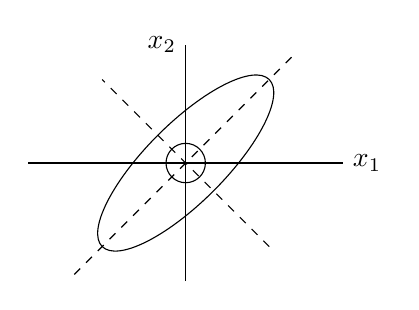
\begin{tikzpicture}
%axis
\draw[](-2,0)--(2,0)node[right]{$x_1$};
\draw[](0,-1.5)--(0,1.5)node[left]{$x_2$};
%
\draw (0,0) circle (0.25);
\draw[rotate=45] (0,0) circle (1.5 and 0.5);
%
\draw[dashed](45:-2)--++(45:4);
\draw[dashed](135:-1.5)--++(135:3);
\end{tikzpicture}
\caption{صدر محور کو نقطہ دار لکیر سے ظاہر کیا گیا ہے۔ (مثال \حوالہ{مثال_امتیازی_جھلی_صدر_محور})}
\label{شکل_مثال_امتیازی_جھلی_صدر_محور}
\end{figure}
\انتہا{مثال}
%=========================
\ابتدا{مثال}\quad امکانی شماریاتی عمل\\
صفحہ \حوالہصفحہ{مثال_خطی_الجبرا_امکانی_شماریاتی_قالب} پر مثال \حوالہ{مثال_خطی_الجبرا_امکانی_شماریاتی_قالب} میں  شہری رقبے کی استعمال کی تقسیم پر غور کیا گیا۔یہ عمل آخر کار  \اصطلاح{تحدیدی حال}\فرہنگ{حال!تحدیدی}\حاشیہب{limit state}\فرہنگ{state!limit} تک پہنچ جائے گا جس کے بعد اس میں مزید تبدیلی رو نما نہیں ہو گی۔یوں امکانی شماریاتی قالب \عددی{\bM{A}\bm{x}=\bM{x}} پر پورا اترے گا۔اس مساوات کی امتیازی قدر اکائی ہے جبکہ امتیازی سمتیہ \عددی{\bM{x}} درکار رقبے کی حتمی تقسیم ہے۔ یوں ہم  \عددی{\bM{A}} سے رو نما ہونے والے عمل کی طویل مدتی اثرات جان سکتے ہیں۔ 

اس مثال میں 
\begin{align*}
\bM{A}=\begin{bmatrix}
0.8&0.1&0\\0.2&0.7&0.1\\0&0.2&0.9
\end{bmatrix}
\end{align*}
ہے جس کے امتیازی اقدار \عددی{\tfrac{7-\sqrt{2}}{10}}، \عددی{\tfrac{7+\sqrt{2}}{10}} اور \عددی{1} ہیں۔ہمیں اکائی امتیازی قدر \عددی{\lambda=1} سے غرض ہے جو \عددی{[1\,\,2\,\,4]^T} ہے۔یوں شہر میں آخر کار رہائشی، تجارتی اور صنعتی تقسیم رقبہ بالترتیب \عددی{1}، \عددی{2} اور \عددی{4} تناسب سے ہو گی۔
\انتہا{مثال}
%=============================
\ابتدا{مثال}\شناخت{مثال_امتیازی_لزلی}\quad نمو آبادی کا \اصطلاح{لزلی نمونہ}\\ 
\اصطلاح{لزلی نمونہ}\فرہنگ{لزلی نمونہ}\حاشیہب{Leslie model}\فرہنگ{Leslie model} جو عمر کے لحاض سے آبادی میں اضافہ بتاتا ہے پر غور کرتے ہیں۔لزلی نمونے میں عمر کے لحاض سے آبادی کی گروہ بندی کی جاتی ہے اور نظر عموماً صرف مادہ جانور پر رکھی جاتی ہے۔فرض کریں کہ کسی جانور کی آبادی میں مادہ جانور کی زیادہ سے زیادہ عمر \عددی{12} سال ہے۔ہم مادہ آبادی کو چار سال کے برابر وقفے سے تین گروہوں میں تقسیم کرتے ہیں۔فرض کریں کہ لزلی قالب درج ذیل ہے۔
\begin{align*}
\bM{L}=[l_{jk}]=\begin{bmatrix} 0& 2.3&0.4\\0.6&0&0\\0&0.3&0 \end{bmatrix}
\end{align*}
لزلی قالب میں  \عددی{l_{1k}} سے مراد \عددی{k} گروہ میں رہتے ہوئے  ایک مادہ سے پیدا ہونے والی بیٹیوں کی اوسط تعداد ہے جبکہ گروہ \عددی{j-1} سے گروہ \عددی{j} تک زندہ پہنچنے والی مادہ کی تناسب کو \عددی{l_{j,j-1}(j=2,3)} سے ظاہر کیا جاتا ہے۔پہلی چار سال کی عمر میں کم عمری کی بنا مادہ بچہ نہیں دیتی لہٰذا \عددی{l_{11}=0} ہے۔اسی طرح پانچ تا آٹھ سال کی عمر میں جوان مادہ زیادہ سے زیادہ (اوسطاً \عددی{2.3}) بچے  دیتی ہے جبکہ ضعیفی  میں مادہ  اوسطاً \عددی{0.4} بچے دیتی ہے۔اسی طرح بچوں کا \عددی{0.6} حصہ یعنی \عددی{\SI{60}{\percent}}  جوانی تک پہنچ پاتا ہے جبکہ جوان جانوروں کا \عددی{0.3} حصہ یعنی \عددی{\SI{30}{\percent}} بڑھاپے تک پہنچتا ہے۔ 

 (الف) اگر ہر گروہ  کی ابتدائی مادہ  آبادی \عددی{2600} ہو تب \عددی{4}، \عددی{8} اور \عددی{12} سال بعد ان گروہوں کی مادہ آبادی کیا ہو گی؟ (ب)  ان گروہوں کی ابتدائی آبادی کیا ہونے سے تمام گروہوں میں تبدیلی کی تناسب برابر ہو گی؟ یہ تناسب کیا ہو گی؟

حل: (الف) ابتدائی طور پر \عددی{\bM{x}_0=[2600\,\,\,\,,2600\,\,\,\,2600]^T} ہے۔چار سال بعد گروہ بندی درج ذیل ہو گی۔
\begin{align*}
\bM{x}_4=\bM{L}\bM{x}_0=\begin{bmatrix} 0& 2.3&0.4\\0.6&0&0\\0&0.3&0 \end{bmatrix}\begin{bmatrix}2600\\2600\\2600  \end{bmatrix}=
\begin{bmatrix}7020\\1560\\780  \end{bmatrix}
\end{align*}
اسی طرح آٹھ سال بعد آبادی \عددی{\bM{x}_8=\bM{L}\bM{x}_4=\bM{L}^2\bM{x}_0=[3900\,\,\,\,4212\,\,\,\,468]^T} اور بارہ سال بعد آبادی
 \عددی{\bM{x}_{12}=\bM{L}\bM{x}_8=\bM{L}^3\bM{x}_0=[9875\,\,\,\, 2340\,\,\,\,1264]^T} ہو گی۔

(ب) متناسب تبدیلی آبادی دریافت کرنے کی خاطر ہمیں ایسا امتیازی سمتیہ \عددی{\bM{x}} درکار ہے جو  \عددی{\bM{L}\bM{x}=\lambda\bM{x}} پر پورا اترتا ہو جہاں \عددی{\lambda>1} آبادی میں اضافے کے تناسب اور \عددی{\lambda<1} آبادی میں کمی کے تناسب کو ظاہر کرے گا۔امتیازی مساوات لکھتے ہیں
\begin{align*}
\begin{vmatrix} -\lambda& 2.3&0.4\\0.6&-\lambda&0\\0&0.3&-\lambda \end{vmatrix}=-\lambda^3+1.38\lambda+0.072=0
\end{align*}
جس کے امتیازی اقدار \عددی{\tfrac{6}{5}}، \عددی{-\tfrac{\sqrt{30}+6}{10}} اور \عددی{\tfrac{\sqrt{30}-6}{10}} ہیں جنہیں کمپیوٹر کی مدد سے حاصل کیا جا سکتا ہے۔امتیازی قدر \عددی{\lambda=\tfrac{6}{5}=1.2} آبادی میں اضافے کو ظاہر کرتی ہے جس کا مطابقتی امتیازی سمتیہ درج ذیل ہے
\begin{align*}
\bM{L}\bM{x}-\lambda \bM{x}=\begin{bmatrix} -1.2&2.3&0.4\\0.6&-1.2&0\\0&0.3&-1.2 \end{bmatrix}\begin{bmatrix}x_1\\x_2\\x_3  \end{bmatrix}=0\quad \implies \quad \bM{x}=\begin{bmatrix} 8\\4\\1 \end{bmatrix}
\end{align*}
جہاں \عددی{x_3=1} چنتے ہوئے \عددی{x_2=4} اور \عددی{x_1=8} حاصل کیا گیا ہے۔ابتدائی کل آبادی \عددی{{3\times 2600=7800}} حاصل کرنے کی خاطر ہم اس امتیازی سمتیہ کو \عددی{\tfrac{7800}{8+4+1}=600} سے ضرب دیتے ہوئے ابتدائی آبادی درج ذیل حاصل کرتے ہیں۔
\begin{align*}
600[8\,\,\,\,4\,\,\,\,1]^T=[4800\,\,\,\,2400\,\,\,\,600]^T
\end{align*}
 آبادی میں تبدیلی کا تناسب \عددی{1.2} فی  چار سال ہو گا۔
\انتہا{مثال}
%===================================

\حصہء{سوالات}
%=============
سوال \حوالہ{سوال_امتیازی_تبدیلی_شکل_الف} تا سوال \حوالہ{سوال_امتیازی_تبدیلی_شکل_ب} میں تبدیلی شکل \عددی{\bM{y}=\bM{A}\bM{x}} کا قالب \عددی{\bM{A}} دیا گیا ہے۔صدر سمتیں اور ان کی مطابقتی سکڑاو یا پھیلاو کا تناسب دریافت کریں۔

%===============
\ابتدا{سوال}\شناخت{سوال_امتیازی_تبدیلی_شکل_الف}\quad
$\begin{bmatrix} 5&2\\2&5 \end{bmatrix}$\\
جوابات:
$3,\, [1\,\,-1]^T, \,\,-45^{\circ};\quad 7,\,[1\,\,1]^T,\,\,45^{\circ}$
\انتہا{سوال}
%===================================
\ابتدا{سوال}\quad
$\begin{bmatrix} 9&8\\8&2 \end{bmatrix}$\\
جوابات:
$-3.23,\, [1\,\,-1.529]^T, \,\,-56.8^{\circ};\quad 14.23,\,[1\,\,0.654]^T,\,\,33.2^{\circ}$
\انتہا{سوال}
%====================================================
\ابتدا{سوال}\quad
$\begin{bmatrix} 1&2\\4&1 \end{bmatrix}$\\
جوابات:
$1-2\sqrt{2},\, [1\,\,-\sqrt{2}]^T, \,\,-54.7^{\circ};\quad 1+2\sqrt{2},\,[1\,\,\sqrt{2}]^T,\,\,54.7^{\circ}$
\انتہا{سوال}
%========================
\ابتدا{سوال}\quad
$\begin{bmatrix} 2&3\\43&12 \end{bmatrix}$\\
جوابات:
$7-\sqrt{34},\, [1\,\,\,\,\tfrac{5-\sqrt{34}}{3}]^T, \,\,-15.5^{\circ};\quad 7+\sqrt{34},\,[1\,\,\,\,\tfrac{5+\sqrt{34}}{3}]^T,\,\,74.5^{\circ}$
\انتہا{سوال}
%=========================
\ابتدا{سوال}\quad
$\begin{bmatrix} 3&1\\5&7 \end{bmatrix}$\\
جوابات:
$2,\, [1\,\,\,\,-1]^T, \,\,-45^{\circ};\quad 8,\,[1\,\,\,\,5]^T,\,\,78.7^{\circ}$
\انتہا{سوال}
%=========================
\ابتدا{سوال}\شناخت{سوال_امتیازی_تبدیلی_شکل_ب}\quad
$\begin{bmatrix} 1.25&0.45\\0.75&2.5 \end{bmatrix}$\\
جوابات:
$1.02,\, [1\,\,\,\,-0.507]^T, \,\,-26.9^{\circ};\quad 2.73,\,[1\,\,\,\,3.285]^T,\,\,73.1^{\circ}$
\انتہا{سوال}
%================================
سوال \حوالہ{سوال_امتیازی_امکانی_شماریاتی_الف} تا سوال \حوالہ{سوال_امتیازی_امکانی_شماریاتی_ب} میں دیے گئے امکانی شماریاتی عمل کا تحدیدی  حال دریافت کریں۔

%===============
\ابتدا{سوال}\شناخت{سوال_امتیازی_امکانی_شماریاتی_الف}\quad
$\begin{bmatrix}0.2&0.5\\0.8&0.5  \end{bmatrix}$\\
جواب:
$\begin{bmatrix}5&8 \end{bmatrix}^T$
\انتہا{سوال}
%===============================
\ابتدا{سوال}\quad
$\begin{bmatrix}0.2&0.5&0.3\\0.3&0.5&0.2 \\0.5&0.2&0.3 \end{bmatrix}$\\
جواب:
$\begin{bmatrix}1&1&1 \end{bmatrix}^T$
\انتہا{سوال}
%===============================
\ابتدا{سوال}\شناخت{سوال_امتیازی_امکانی_شماریاتی_ب}\quad
$\begin{bmatrix}0.4&0.1&0.3\\0.5&0.1&0.2& \\0.1&0.8&0.5 \end{bmatrix}$\\
جواب:
$\begin{bmatrix}29&27&49 \end{bmatrix}^T$
\انتہا{سوال}
%===============================
سوال \حوالہ{سوال_امتیازی_لزلی-الف} اور سوال \حوالہ{سوال_امتیازی_لزلی-ب} میں لزلی نمونے کا قالب \عددی{\bM{L}} دیا گیا ہے (مثال \حوالہ{مثال_امتیازی_لزلی})۔نمو آبادی کا تناسب دریافت کریں۔

%==========
\ابتدا{سوال}\شناخت{سوال_امتیازی_لزلی-الف}\quad
$\begin{bmatrix}0&3.45&0.6\\0.9&0&0\\0&0.45&0 \end{bmatrix}$\\
جواب:\عددی{\tfrac{9}{5}}
\انتہا{سوال}
%==========================
\ابتدا{سوال}\شناخت{سوال_امتیازی_لزلی-ب}\quad
$\begin{bmatrix}0&9&5\\0.4&0&0\\0&0.4&0 \end{bmatrix}$\\
جواب:\عددی{2}
\انتہا{سوال}
%========================
سوال \حوالہ{سوال_امتیازی_لیونٹف_الف} تا سوال \حوالہ{سوال_امتیازی_لیونٹف_ب}  \اصطلاح{لیونٹف  نمونہ}\فرہنگ{لیونٹف نمونہ}\فرہنگ{نمونہ!لیونٹف}\حاشیہب{Leontief model}\فرہنگ{model!Leontief} برائے مدخل و مخرج پر مبنی ہیں۔

%===============
\ابتدا{سوال}\شناخت{سوال_امتیازی_لیونٹف_الف}
\اصطلاح{لیونٹف مدخل و مخرج نمونہ}\حاشیہد{روس کے وسیلی وسیلی وچ لیونٹف [1906-1999] نے یہ نمونہ پیش کر کے نوبل انعام حاصل کیا۔} صنعت کی پیداوار اور اس کے اخراجات کا تعلق بیان کرتا ہے۔فرض کریں کہ تین صنعتوں کی پیداوار یہی صنعت استعمال کرتے ہیں اور اس تعلق کو درج ذیل \عددی{3\times 3} \اصطلاح{قالب صرف}\فرہنگ{قالب صرف}\حاشیہب{consumption matrix}\فرہنگ{matrix!consumption}  پیش کرتا ہے
\begin{align*}
\bM{A}=[a_{jk}]=\begin{bmatrix} 0.1&0.5&0\\0.8&0&0.4\\0.1&0.5&0.6 \end{bmatrix}
\end{align*}
جہاں \عددی{a_{jk}} صنعت \عددی{k} کی پیداوار کی وہ تناسب  ہے جو صنعت \عددی{j} خرید کر استعمال کرتی ہے۔ فرض کریں کہ صنعت \عددی{j} کی کل پیداوار کی آمدن \عددی{p_j}  ہے۔ہم چاہتے ہیں کہ ایسی قیمتیں دریافت کریں کہ ہر صنعت کی اخراجات اس صنعت کی آمدی کے برابر ہو۔ اس کو بطور مسئلہ \عددی{\bM{A}\bM{p}=\bM{p}} لکھا جا سکتا ہے جہاں \عددی{\bM{p}=[p_1\,\,\,p_2\,\,\,p_3]^T} ہے۔ایسا \عددی{\bM{p}} دریافت کریں کہ \عددی{p_1}، \عددی{p_2} اور \عددی{p_3} غیر منفی ہوں۔

جواب:
$c[10\quad 18\quad 25]^T$
جہاں \عددی{c} مستقل ہے۔
\انتہا{سوال}
%========================
\ابتدا{سوال}
ثابت کریں کہ سوال \حوالہ{سوال_امتیازی_لیونٹف_الف} کے قالب صرف  کے ہر قطار کے ارکان کا مجموعہ اکائی (\عددی{1}) ہو گا اور اس قالب صرف کا امتیازی قدر بھی اکائی ہو گا۔
\انتہا{سوال}
%==============================
\ابتدا{سوال}\شناخت{سوال_امتیازی_لیونٹف_ب}
آزاد لیونٹف نمونے میں پیداوار کا کچھ حصہ یہی صنعت استعمال کرتے ہیں جبکہ باقی حصہ فروخت کیا جاتا ہے۔یوں \عددی{\bM{A}\bM{x}=\bM{x}} (سوال \حوالہ{سوال_امتیازی_لیونٹف_الف}) کی بجائے،   \عددی{\bM{x}-\bM{A}\bM{x}=\bM{y}} ہو گا جہاں \عددی{\bM{x}} پیداوار ہے جبکہ \عددی{\bM{A}\bM{x}} وہ حصہ ہے جو یہی صنعتیں خود استعمال کرتی ہیں لہٰذا \عددی{\bM{y}} وہ حصہ ہے جس کو فروخت کیا جا سکتا ہے۔

\اصطلاح{قالب مانگ}\فرہنگ{قالب!مانگ}\فرہنگ{مانگ!قالب}\حاشیہب{demand matrix}\فرہنگ{matrix!demand}\فرہنگ{demand!matrix}
 \عددی{\bM{y}=[0.1\,\,\,\,0.3\,\,\,\,0.1]^T} کو پورا کرنے کے لئے قالب پیداوار \عددی{\bM{x}} دریافت کریں جہاں قالب صرف درج ذیل ہے۔
\begin{align*}
\bM{A}=\begin{bmatrix} 0.1&0.4&0.2\\0.5&0&0.1\\0.1&0.4&0.4 \end{bmatrix}
\end{align*}
جواب:
$\bM{x}=(\bM{I}-\bM{A})^{-1}\bM{y}=[0.6747\,\,\,\,0.7128\,\,\,\,0.7543]^T$
\انتہا{سوال}
%=================================
سوال \حوالہ{سوال_امتیازی_عمومی_خصوصیات_الف} تا سوال \حوالہ{سوال_امتیازی_عمومی_خصوصیات_ب} امتیازی قدر مسائل کے عمومی خصوصیات پر مبنی ہیں جنہیں آپ نے ثابت کرنا ہے۔ان مسائل میں فرض کریں کہ \عددی{n\times n} قالب \عددی{\bM{A}} کے امتیازی اقدار \عددی{\lambda_1} تا  \عددی{\lambda_n} ہیں جو غیر منفرد ہو سکتے ہیں۔

%===============
\ابتدا{سوال}\شناخت{سوال_امتیازی_عمومی_خصوصیات_الف}
مرکزی وتر کے ارکان کا مجموعہ اور امتیازی اقدار کا مجموعہ برابر ہیں۔
\انتہا{سوال}
%====================
\ابتدا{سوال}\quad طیفی منتقلی\\
\عددی{\bM{A}-k\bM{I}} کے امتیازی اقدار \عددی{\lambda_1-k} تا  \عددی{\lambda_n-k} ہیں جبکہ اس کے امتیازی سمتیات وہی ہیں جو \عددی{\bM{A}} کے امتیازی سمتیات ہیں۔
\انتہا{سوال}
%=========================
\ابتدا{سوال}\شناخت{سوال_امتیازی_غیر_سمتی_ضرب_طاقت}\quad غیر سمتی مضرب، طاقت\\
غیر سمتی مضرب \عددی{k\bM{A}} کے امتیازی اقدار \عددی{k\lambda_1} تا \عددی{k\lambda_n} ہیں جبکہ \عددی{\bM{A}^m} جہاں \عددی{m=1,2,\cdots} ہے کے امتیازی اقدار \عددی{\lambda_1^m} تا \عددی{\lambda_n^m} ہیں۔دونوں صورتوں میں امتیازی سمتیات وہی ہیں جو \عددی{\bM{A}} کے امتیازی سمتیات ہیں۔
\انتہا{سوال}
%=========================
\ابتدا{سوال}\شناخت{سوال_امتیازی_عمومی_خصوصیات_ب}
کثیر رکنی \عددی{p(\bM{A})=k_m\bM{A}^m+k_{m-1}\bM{A}^{m-1}+\cdots+k_1\bM{A}+k_0\bM{I}} کے امتیازی اقدار درج ذیل ہیں
\begin{align*}
p(\lambda_j)=k_j\lambda_j^m+k_{m-1}\lambda_j^{m-1}+\cdots+k_1\lambda_j+k_0
\end{align*}
جہاں \عددی{j=1,2,\cdots} ہے جبکہ اس کثیر رکنی کے امتیازی سمتیات وہی ہیں کو \عددی{\bM{A}} کے امتیازی سمتیات ہیں۔(سوال \حوالہ{سوال_امتیازی_غیر_سمتی_ضرب_طاقت} کے نتائج استعمال کریں۔)
\انتہا{سوال}
%=================================

\حصہ{تشاکلی، منحرف تشاکلی اور قائمہ الزاویہ قالب}\شناخت{حصہ_امتیازی_تشاکلی_منحرف_قائمہ}
حقیقی چکور قالب کی تین اقسام پر یہاں غور کیا جائے گا جن کی غیر معمولی خصوصیات پائی جاتی ہیں۔تشاکلی اور منحرف تشاکلی قالب کا حصہ \حوالہ{حصہ_الجبرا_قالبی_ضرب} میں ذکر ہو چکا ہے۔

%============
\ابتدا{تعریف}\quad تشاکلی، منحرف تشاکلی اور قائمہ الزاویہ قالب\\
ایسا \اصطلاح{حقیقی} چکور قالب \عددی{\bM{A}=[a_{jk}]} جو تبدیلی محل سے  تبدیل نہیں ہوتا \اصطلاح{تشاکلی}\فرہنگ{تشاکلی}\حاشیہب{symmetric}\فرہنگ{symmetric} قالب کہلاتا ہے۔
\begin{align}\label{مساوات_امتیازی_تشاکل_منحرف_تشاکل_قائمہ_الف}
\bM{A}^T=\bM{A} \quad \implies \quad [a_{kj}]=[a_{jk}]
\end{align}
ایسا \اصطلاح{حقیقی} چکور قالب \عددی{\bM{A}=[a_{jk}]} جس کا تبدیل محل اس قالب کا منفی  ہو \اصطلاح{منحرف تشاکلی}\فرہنگ{منحرف تشاکلی}\حاشیہب{skew-symmetric}\فرہنگ{skew-symmetric} قالب کہلاتا ہے۔
\begin{align}\label{مساوات_امتیازی_تشاکل_منحرف_تشاکل_قائمہ_ب}
\bM{A}^T=-\bM{A}\quad \implies \quad [a_{kj}]=-[a_{jk}]
\end{align}
ایسا \اصطلاح{حقیقی} چکور قالب \عددی{\bM{A}=[a_{jk}]} جس کا تبدیل محل اس  قالب کا معکوس ہو  \اصطلاح{قائمہ الزاویہ}\فرہنگ{قائمہ الزاویہ}\حاشیہب{orthogonal}\فرہنگ{orthogonal} قالب کہلاتا ہے۔
\begin{align}\label{مساوات_امتیازی_تشاکل_منحرف_تشاکل_قائمہ_پ}
\bM{A}^T=\bM{A}^{-1}
\end{align}
\انتہا{تعریف}
%======================
\ابتدا{مثال}\شناخت{مثال_امتیازی_تشاکلی_منحرف_قائمہ}\quad تشاکلی، منحرف تشاکلی اور قائمہ الزاویہ قالب\\
آپ سے التماس ہے کہ درج ذیل میں تشاکلی، منحرف تشاکلی اور قائمہ الزاویہ قالب کی پہچان کریں۔
\begin{align*}
\begin{bmatrix*}[r] 1&-3&2\\-3&4&-7\\2&-7&0 \end{bmatrix*},\quad \begin{bmatrix*}[r] 0&-1&2\\1&0&-4\\-2&4&0 \end{bmatrix*},\quad
\begin{bmatrix*}[r] \tfrac{2}{3}&\tfrac{1}{3}&\tfrac{2}{3}\\-\tfrac{2}{3}&\tfrac{2}{3}&\tfrac{1}{3}\\ \tfrac{1}{3}&\tfrac{2}{3}&-\tfrac{2}{3} \end{bmatrix*}
\end{align*}
کیا آپ ثابت کر سکتے ہیں کہ ہر منحرف تشاکلی قالب کے مرکزی وتر کے تمام اجزاء صفر ہوں گے؟
\انتہا{مثال}
%======================

کسی بھی حقیقی چکور قالب کو تشاکلی قالب \عددی{\bM{R}} اور منحرف تشاکلی قالب \عددی{\bM{S}} کا مجموعہ لکھا جا سکتا ہے جہاں تشاکلی قالب اور منحرف تشاکلی قالب درج ذیل ہیں۔
\begin{align}
\bM{R}=\frac{1}{2}(\bM{A}+\bM{A}^T),\quad \bM{S}=\frac{1}{2}(\bM{A}-\bM{A}^T)
\end{align}
%===================
\ابتدا{مثال}\quad قالب بطور تشاکلی اور منحرف تشاکلی قالب کا مجموعہ\\
\begin{align*}
\bM{A}=\begin{bmatrix*}[r] 4&2&-1\\2&8&3\\5&1&3 \end{bmatrix*}=\bM{R}+\bM{S}=\begin{bmatrix*}[r]4&2&2\\2&8&2\\2&2&3  \end{bmatrix*}+\begin{bmatrix*}[r] 0&0&-3\\0&0&1\\3&-1&0  \end{bmatrix*}
\end{align*}
\انتہا{مثال}
%================================

\ابتدا{مسئلہ}\شناخت{مسئلہ_امتیازی_تشاکلی_منحرف_تشاکلی_اقدار}\quad تشاکلی اور منحرف تشاکلی قالب کے امتیازی اقدار\\
(الف) تشاکلی قالب کے امتیازی اقدار حقیقی ہوں گے۔\\
(ب) منحرف تشاکلی قالب کے امتیازی اقدار خیالی یا صفر ہوں گے۔ 
\انتہا{مسئلہ}
%===========================

درج بالا مسئلے کا ثبوت مسئلہ \حوالہ{مسئلہ_امتیازی_ہرمشی_منحرف_ہرمشی_اکہرا_امتیازی_اقدار} میں پیش کیا جائے گا۔

%=================
\ابتدا{مثال}\quad تشاکلی اور منحرف تشاکلی قالب کے امتیازی اقدار\\
درج ذیل تشاکلی قالب \عددی{R} کے امتیازی اقدار \عددی{-2} اور \عددی{4} ہیں جبکہ منحرف تشاکلی قالب \عددی{S} کے امتیازی اقدار \عددی{-3i} اور \عددی{3i} ہیں۔قالب \عددی{\bM{C}} نا تشاکلی اور نا منحرف تشاکلی ہے جبکہ اس کے امتیازی اقدار \عددی{0} اور \عددی{4} ہیں۔مسئلہ \حوالہ{مسئلہ_امتیازی_تشاکلی_منحرف_تشاکلی_اقدار} ایسے قالب کے بارے میں کچھ نہیں کہتا ہے۔
\begin{align*}
\bM{R}=\begin{bmatrix*}[r]1&3\\3&1  \end{bmatrix*}, \quad\bM{S}=\begin{bmatrix*}[r] 0&3\\-3&0\end{bmatrix*},\quad \bM{C}=\begin{bmatrix}2&4\\1&2  \end{bmatrix}
\end{align*}
\انتہا{مثال}
%======================

\جزوحصہء{قائمہ الزاویہ تبادلے اور قائمہ الزاویہ قالب}
قائمہ الزاویہ تبادلے سے مراد درج ذیل ہے جہاں \عددی{\bM{A}} قائمہ الزاویہ قالب ہے۔
\begin{align}
\bM{y}=\bM{A}\bM{x}
\end{align}
 قائمہ الزاویہ تبادلہ \عددی{R^n} میں ہر سمتیہ \عددی{\bM{x}} کی جگہ \عددی{R^n} میں سمتیہ \عددی{\bM{y}} مقرر کرتا ہے۔مثال کے طور پر سطح میں گھومنا، قائمہ الزاویہ تبادل ہے یعنی:
\begin{align}\label{مساوات_امتیازی_سطحی_گردش}
\bM{y}=\begin{bmatrix} y_1\\y_2 \end{bmatrix}=\begin{bmatrix*}[r] \cos \theta&-\sin \theta\\ \sin \theta &\cos \theta \end{bmatrix*}\begin{bmatrix}x_1\\x_2  \end{bmatrix}
\end{align}
یہ ثابت کیا جا سکتا ہے سطح یا تین بعدی فضا میں قائمہ الزاویہ تبادل \اصطلاح{گھومنے} کو ظاہر کرتا ہے (اور ساتھ ہی بالترتیب کسی خط یا سطح میں انعکاس بھی ممکن ہے)۔

قائمہ الزاویہ قالب کی اہمیت درج ذیل کی بنا ہے۔
%====================
\ابتدا{مسئلہ}\شناخت{مسئلہ_امتیازی_اندرونی_ضرب_کی-عدم_تغیر_الف}\quad اندرونی ضرب کی عدم تغیر\\
\عددی{R^n} میں سمتیات \عددی{\bM{a}} اور \عددی{\bM{b}} کے \اصطلاح{اندرونی ضرب}\فرہنگ{اندرونی!ضرب} کی قیمت کو قائمہ الزاویہ تبادل  برقرار رکھتا ہے جہاں اندرونی ضرب درج ذیل ہے۔
\begin{align}
\bM{a}\cdot \bM{b}=\bM{a}^T\bM{b}=[a_1\,\,\cdots\,\,a_n]\begin{bmatrix}b_1\\  \vdots \\ b_n  \end{bmatrix}
\end{align}
یوں \عددی{n\times n} قائمہ الزاویہ قالب \عددی{\bM{A}} اور \عددی{R^n} میں کسی بھی  \عددی{\bM{a}}، \عددی{\bM{b}} اور \عددی{\bM{u}=\bM{A}\bM{a}}، \عددی{\bM{v}=\bM{A}\bM{b}} کی صورت میں \عددی{\bM{u}\cdot\bM{v}=\bM{a}\cdot\bM{b}} ہو گا۔

اس طرح  \عددی{R^n} میں ہر سمتیہ \عددی{\bM{a}} کی \اصطلاح{لمبائی}\فرہنگ{لمبائی} یا \اصطلاح{معیار}\فرہنگ{معیار} کو قائمہ الزاویہ تبادل برقرار رکھتا ہے جہاں سمتیہ کی لمبائی یا معیار درج ذیل ہے۔
\begin{align}
\norm{\bM{a}}=\sqrt{\bM{a}\cdot \bM{a}}=\sqrt{\bM{a}^T\bM{a}}
\end{align}  
\انتہا{مسئلہ}
%=======================

\ابتدا{ثبوت}
فرض کریں کہ \عددی{\bM{A}} قائمہ الزاویہ ہے اور  \عددی{\bM{u}=\bM{A}\bM{a}}، \عددی{\bM{v}=\bM{A}\bM{b}} ہیں۔اب صفحہ \حوالہصفحہ{مساوات_الجبرا_تبدیل_محل_قواعد} پر مساوات \حوالہ{مساوات_الجبرا_تبدیل_محل_قواعد}-ت کے تحت \عددی{(\bM{A}\bM{a})^T=\bM{a}^T\bM{A}^T} ہو گا جبکہ مساوات \حوالہ{مساوات_امتیازی_تشاکل_منحرف_تشاکل_قائمہ_پ} کے تحت \عددی{\bM{A}^T\bM{A}=\bM{A}^{-1}\bM{A}=\bM{I}} ہو گا۔اس طرح درج ذیل لکھا جا سکتا ہے۔
\begin{align}
\bM{u}\cdot \bM{v}=\bM{u}^T\bM{v}=(\bM{A}\bM{a})^T\bM{A}\bM{b}=\bM{a}^T\bM{A}^T\bM{A}\bM{b}=\bM{a}^T\bM{I}\bM{b}=\bM{a}^T\bM{b}=\bM{a}\cdot\bM{b}
\end{align} 
اس میں \عددی{\bM{b}=\bM{a}} پر کرنے سے \عددی{\norm{\bM{a}}} عدم تغیر ثابت ہوتا ہے۔
\انتہا{ثبوت}
%=============================

\ابتدا{مسئلہ}\شناخت{مسئلہ_امتیازی_صف_قطار_قائمیت}\quad صف اور قطار کی معیاری قائمیت\\
حقیقی چکور قالب صرف اور صرف اس صورت قائمہ الزاویہ ہو گا جب اس کے سمتیات قطار \عددی{\bM{a}_1} تا \عددی{\bM{a}_n} (اور سمتیات صف) معیاری قائمہ الزاویہ ہوں یعنی:
\begin{align}\label{مساوات_امتیازی_معیاری_قائمیت_الف}
\bM{a}_j\cdot\bM{a}_k=\bM{a}^T\bM{a}_k=
\begin{cases}
0& j\ne k\\
1&j=k
\end{cases}
\end{align}
\انتہا{مسئلہ}
%==============================

\ابتدا{ثبوت}
(الف) فرض کریں کہ \عددی{\bM{A}} قائمہ الزاویہ ہے۔یوں \عددی{\bM{A}^{-1}\bM{A}=\bM{A}^T\bM{A}=\bM{I}} ہو گا جس کو سمتیات قطار \عددی{\bM{a}_1} تا \عددی{\bM{a}_n} کی صورت میں لکھتے ہیں۔
\begin{align}\label{مساوات_امتیازی_معیاری_قائمیت_ب}
\bM{I}=\bM{A}^{-1}\bM{A}=\bM{A}^T\bM{A}=\begin{bmatrix}\bM{a}_1^T\\  \vdots \\ \bM{a}_n^T  \end{bmatrix}\begin{bmatrix} \bM{a}_1 \cdots \bM{a}_n \end{bmatrix}=
\begin{bmatrix} \bM{a}_1^T\bM{a}_1&\bM{a}_1^T\bM{a}_2&\cdots&\bM{a}_1^T\bM{a}_n\\  \vdots \\ 
\bM{a}_n^T\bM{a}_1&\bM{a}_n^T\bM{a}_2&\cdots&\bM{a}_n^T\bM{a}_n \end{bmatrix}
\end{align}
چونکہ \عددی{n\times n} اکائی قالب \عددی{\bM{I}} کا مرکزی وتر اکائی جبکہ باقی تمام اجزاء صفر ہوتے ہیں لہٰذا مساوات \حوالہ{مساوات_امتیازی_معیاری_قائمیت_ب} کا دائیں ہاتھ  مساوات \حوالہ{مساوات_امتیازی_معیاری_قائمیت_الف} دیتا ہے۔مساوات \حوالہ{مساوات_امتیازی_تشاکل_منحرف_تشاکل_قائمہ_پ} کے تحت قائمہ الزاویہ قالب کا معکوس بھی قائمہ الزاویہ ہو گا۔ اب \عددی{\bM{A}^{-1}(=\bM{A}^T)} کے سمتیات قطار \عددی{\bM{A}} کے سمتیات صف ہیں لہٰذا \عددی{\bM{A}} کے سمتیات صف بھی قائمہ الزاویہ ہوں گے۔ 

(ب) اس کے برعکس اگر \عددی{\bM{A}} کے سمتیات قطار مساوات \حوالہ{مساوات_امتیازی_معیاری_قائمیت_الف} پر پورا اترتے ہوں تب مساوات \حوالہ{مساوات_امتیازی_معیاری_قائمیت_ب} دائیں ہاتھ قالب کے مرکزی وتر سے ہٹ کر تمام ارکان صفر \عددی{(0)} ہوں گے جبکہ وتری ارکان اکائی \عددی{(1)} ہوں گے لہٰذا \عددی{\bM{A}^T\bM{A}=\bM{I}} ہو گا۔اسی طرح \عددی{\bM{A}\bM{A}^T=\bM{I}} ہو گا۔ اس سے مراد \عددی{\bM{A}^T=\bM{A}^{-1}} ہے چونکہ \عددی{\bM{A}^{-1}\bM{A}=\bM{A}\bM{A}^{-1}=\bM{I}} ہے جبکہ \عددی{\bM{A}^{-1}} یکتا  ہے۔یوں \عددی{\bM{A}} قائمہ الزاویہ ہو گا۔ثبوت کے حصہ-الف کے آخر کی طرح \عددی{\bM{A}} کے سمتیات قطار بھی قائمہ الزاویہ ہوں گے۔
\انتہا{ثبوت}
%===========================

\ابتدا{مسئلہ}\شناخت{مسئلہ_امتیازی_قائمہ_مقطع_اکائی}\quad قائمہ الزاویہ قالب کا مقطع\\
قائمہ الزاویہ قالب کی مقطع کی قیمت \عددی{+1} یا \عددی{-1} ہو گی۔
\انتہا{مسئلہ}
%===============================

\ابتدا{ثبوت}
صفحہ \حوالہصفحہ{مسئلہ_خطی_الجبرا_مقطع_حاصل_ضرب} پر مسئلہ \حوالہ{مسئلہ_خطی_الجبرا_مقطع_حاصل_ضرب} کے تحت  درج ذیل ہے
\begin{align*}
(\bM{AB})\,\text{مقطع}=(\bM{A}\,\text{مقطع})(\bM{B}\,\text{مقطع})
\end{align*}
جبکہ صفحہ \حوالہصفحہ{مسئلہ_الجبرا_مقطع_خصوصیات_مزید} پر مسئلہ \حوالہ{مسئلہ_الجبرا_مقطع_خصوصیات_مزید}-ت کے تحت
$\bM{A}\,\text{مقطع}=\bM{A}^T\,\text{مقطع}$
ہے لہٰذا قائمہ الزاویہ قالب کے لئے درج ذیل ہو گا۔
\begin{align}
1=\bM{I}\,\text{مقطع}=(\bM{A}\bM{A}^{-1})\,\text{مقطع}=(\bM{A}\bM{A}^T)\,\text{مقطع}=(\bM{A}\,\text{مقطع})(\bM{A}^T\,\text{مقطع})=(\bM{A}\,\text{مقطع})^2
\end{align}
\انتہا{ثبوت}
%===============================

\ابتدا{مثال}\quad مسئلہ \حوالہ{مسئلہ_امتیازی_قائمہ_مقطع_اکائی}\\
مثال \حوالہ{مثال_امتیازی_تشاکلی_منحرف_قائمہ} میں دیے گئے قائمہ الزاویہ قالب کا مقطع \عددی{-1} ہے جبکہ  مساوات \حوالہ{مساوات_امتیازی_سطحی_گردش} کے قالب کا مقطع \عددی{+1} ہے۔
\انتہا{مثال}
%=============================

\ابتدا{مسئلہ}\شناخت{مسئلہ_امتیازی_قائمہ_اکائی_حتمی}\quad قائمہ الزاویہ قالب کے امتیازی اقدار\\
قائمہ الزاویہ قالب کے امتیازی اقدار حقیقی یا جوڑی دار مخلوط ہوں گے جن کی حتمی قیمت اکائی ہو گی۔
\انتہا{مسئلہ}
%================================

\ابتدا{ثبوت}
چونکہ حقیقی قالب کی امتیازی کثیر رکنی کے عددی سر حقیقی ہوتے ہیں لہٰذا اس کے امتیازی اقدار (یعنی صفر) مسئلے کے تحت ہوں گے۔یوں مسئلے کا پہلا حصہ کسی بھی  حقیقی قالب کے لئے درست ہے۔امتیازی قدر کی حتمی قیمت اکائی کے برابر \عددی{\abs{\lambda}=1} ہونے کا ثبوت مسئلہ \حوالہ{مسئلہ_امتیازی_ہرمشی_منحرف_ہرمشی_اکہرا_امتیازی_اقدار} میں پیش کیا جائے گا۔
\انتہا{ثبوت}
%=============================

\ابتدا{مثال}
مثال \حوالہ{مثال_امتیازی_تشاکلی_منحرف_قائمہ} میں دیے گئے قائمہ الزاویہ قالب کی امتیازی کثیر رکنی درج ذیل ہے۔
\begin{align*}
-\lambda^3+\frac{2}{3}\lambda^2+\frac{2}{3}\lambda-1=0
\end{align*} 
چونکہ مخلوط جذر صرف جوڑی دار ممکن ہیں لہٰذا اس کثیر رکنی کا ایک جذر حقیقی ہو گا جو مسئلہ \حوالہ{مسئلہ_امتیازی_قائمہ_مقطع_اکائی} کے تحت \عددی{+1} یا \عددی{-1} ہو گا۔ان قیمتوں کو کثیر رکنی میں پر کرتے ہوئے پہلا جذر یعنی امتیازی اقدار \عددی{\lambda=-1} ملتا ہے۔کثیر رکنی کو \عددی{\lambda+1} سے تقسیم کرتے ہوئے \عددی{-(\lambda^2-\tfrac{5}{3}\lambda+1)=0} ملتا ہے جس کے جذر  \عددی{\tfrac{5+i\sqrt{11}}{6}} اور \عددی{\tfrac{5-i\sqrt{11}}{6}} ہیں جن کی حتمی قیمت \عددی{1} ہے۔
\انتہا{مثال}
%==========================

\حصہء{سوالات}
سوال \حوالہ{سوال_امتیازی_طیف_الف} تا سوال \حوالہ{سوال_امتیازی_طیف_ب} میں قالب تشاکلی، منحرف تشاکلی یا قائمہ الزاویہ ہیں؟ ان کا طیف  دریافت کریں جو مسئلہ \حوالہ{مسئلہ_امتیازی_تشاکلی_منحرف_تشاکلی_اقدار} اور مسئلہ \حوالہ{مسئلہ_امتیازی_قائمہ_اکائی_حتمی} پر پورا اتریں گے۔ امتیازی سمتیات بھی معلوم کریں۔

%============
\ابتدا{سوال}\شناخت{سوال_امتیازی_طیف_الف}\quad
$\begin{bmatrix*}[r] 0.8&0.6\\-0.6&0.8 \end{bmatrix*}$\\
جوابات:قائمہ الزاویہ،
$\tfrac{4-i3}{5}, \,\, [1\quad-i]^T; \quad \tfrac{4+i3}{5},\,\, [1\quad i]^T$
\انتہا{سوال}
%=======================
\ابتدا{سوال}\quad
$\begin{bmatrix*}[r] 2&3\\-3&2 \end{bmatrix*}$\\
جوابات:تینوں قسم نہیں ہے، 
$2-i3,\,\, [1\quad -i]^T; \quad 2+i3,\,\,[1\quad i]^T$
\انتہا{سوال}
%=======================
\ابتدا{سوال}\quad
$\begin{bmatrix*}[r] a&b\\-b&a \end{bmatrix*}$\\
جوابات:تینوں قسم نہیں ہے، 
$a-ib,\,\,[1\quad -i]^T;\quad a+ib,\,\,[1\quad i]^T$
\انتہا{سوال}
%=======================
\ابتدا{سوال}\quad
$\begin{bmatrix*}[r] 4&0&0\\0&2&-2\\ 0&-2&5 \end{bmatrix*}$\\
جوابات:تشاکلی، 
$6,\,\,[0\quad 1\quad -2]^T;\quad 1,\,\,[0\quad 1\quad \tfrac{1}{2}]^T;\quad 4,\,\,[1\quad 0\quad 0]^T$
\انتہا{سوال}
%=======================
\ابتدا{سوال}\quad
$\begin{bmatrix*}[r] a&b&b\\b&a&b\\b&b&a \end{bmatrix*}$\\
جوابات:تشاکلی، 
$a+2b,\,\,[1\quad 1\quad 1]^T;\quad a-b,\,\,[1\quad 0\quad-1]^T,\,\,[0\quad 1\quad -1]^T$
\انتہا{سوال}
%=======================
\ابتدا{سوال}\quad
$\begin{bmatrix*}[r] 0&9&-12\\-9&0&20\\12&-20&0 \end{bmatrix*}$\\
جوابات:منحرف تشاکلی، 
$\pm 25i,\,\,[1\,\,\pm\tfrac{16+i15}{15}\,\, \pm\tfrac{12-i20}{15}]^T;\,\, 0,\,\,[0\,\, \tfrac{3}{5}\,\, \tfrac{9}{20}]^T$
\انتہا{سوال}
%=======================
\ابتدا{سوال}\quad
$\begin{bmatrix*}[r] 1&0&0\\0&\sin \theta&\cos \theta\\ 0 &-\cos \theta&\sin \theta \end{bmatrix*}$\\
جوابات:تینوں نہیں، 
$\sin \theta\pm i\cos \theta,\,\,[0\quad 1 \quad \pm i]^T;\quad  1,\,\,[1\quad 0\quad 0]^T$
\انتہا{سوال}
%=======================
\ابتدا{سوال}\quad
$\begin{bmatrix*}[r] \tfrac{4}{9}&\tfrac{8}{9}&\tfrac{1}{9}\\-\tfrac{7}{9}&\tfrac{4}{9}&-\tfrac{4}{9}\\-\tfrac{4}{9}&\tfrac{1}{9}&\tfrac{8}{9} \end{bmatrix*}$\\
جوابات:قائمہ الزاویہ، 
$\tfrac{7\pm i5\sqrt{11}}{18},\,\,[1\quad \tfrac{-1\pm i3\sqrt{11}}{10}\quad \tfrac{3\pm i\sqrt{11}}{10}]^T;\quad  1,\,\,[1\quad 1\quad -3]^T$
\انتہا{سوال}
%=======================
\ابتدا{سوال}\شناخت{سوال_امتیازی_طیف_ب}\quad
$\begin{bmatrix*}[r] 0&0&1\\0&1&0\\ -1&0&0\end{bmatrix*}$\\
جوابات:قائمہ الزاویہ، 
$\pm i,\,\,[1\quad 0 \quad \pm i]^T;\quad  1,\,\,[0\quad 1\quad 0]^T$
\انتہا{سوال}
%=======================
سوال \حوالہ{سوال_امتیازی_عمومی_خاصیت_الف} تا سوال \حوالہ{سوال_امتیازی_عمومی_خاصیت_ب} عمومی خصوصیات پر مبنی ہیں۔

%====================
\ابتدا{سوال}\شناخت{سوال_امتیازی_عمومی_خاصیت_الف}\quad مجموعہ\\
کیا \عددی{\bM{A}+\bM{B}} کے امتیازی اقدار \عددی{\bM{A}} اور \عددی{\bM{B}} کے امتیازی اقدار کا مجموعہ ہوں گے۔

جواب:نہیں
\انتہا{سوال}
%======================
\ابتدا{سوال}\quad ثبوت\\
ثابت کریں کہ تشاکلی قالب کے منفرد امتیازی اقدار کے مطابقتی امتیازی سمتیات قائمہ الزاویہ ہوں گے۔مثال دیں۔
\انتہا{سوال}
%=======================
\ابتدا{سوال}\quad منحرف تشاکلی قالب\\
ثابت کریں کہ منحرف تشاکلی قالب کا معکوس بھی منحرف تشاکلی قالب ہو گا۔

جواب:
$\bM{A}^{-1}=(-\bM{A}^T)^{-1}=-(\bM{A}^{-1})^T$
\انتہا{سوال}
%==========================
\ابتدا{سوال}\شناخت{سوال_امتیازی_عمومی_خاصیت_ب}\quad قائمہ الزاویہ قالب\\
کیا \عددی{3\times 3} منحرف تشاکلی قائمہ الزاویہ قالب موجود ہیں؟
\انتہا{سوال}
%============================

\حصہ{امتیازی اساس، وتری بنانا، دو درجی صورت}\شناخت{حصہ_امتیازی_اساس_دو_درجی}
اب تک امتیازی اقدار کی خصوصیات پر غور کیا گیا۔آئیں اب امتیازی سمتیات کی خصوصیات پر غور کرتے ہیں۔\عددی{n\times n} قالب \عددی{\bM{A}} کے امتیازی سمتیات  کبھی  کبھار فضا \عددی{R^n} کی اساس ہوتے ہیں لہٰذا \عددی{R^n} میں کسی بھی سمتیہ \عددی{\bM{x}} کو ان امتیازی سمتیات \عددی{\bM{x}_1}،\نقطے، \عددی{\bM{x}_n} کا مجموعہ لکھا جا سکتا ہے مثلاً:
\begin{align}
\bM{x}=c_1\bM{x}_1+c_2\bM{x}_2+\cdots+c_n\bM{x}_n
\end{align}
ان امتیازی سمتیات کے مطابقتی امتیازی اقدار (جو ضروری نہیں کہ منفرد ہوں) کو \عددی{\lambda_1} تا \عددی{\lambda_n} سے ظاہر کرتے ہوئے
 \عددی{\bM{A}\bM{x}_j=\lambda_j\bM{x}_j} لکھا جا سکتا ہے لہٰذا تبادلہ \عددی{\bM{y}=\bM{A}\bM{x}} درج ذیل ہو گا۔
\begin{gather}
\begin{aligned}
\bM{y}=\bM{A}\bM{x}&=\bM{A}(c_1\bM{x}_1+c_2\bM{x}_2+\cdots+c_n\bM{x}_n)\\
&=c_1\bM{A}\bM{x}_1+c_2\bM{A}\bM{x}_2+\cdots+c_n\bM{A}\bM{x}_n\\
&=c_1\lambda_1\bM{x}_1+c_2\lambda_2\bM{x}_2+\cdots+c_n\lambda_n\bM{x}_n
\end{aligned}
\end{gather}
آپ دیکھ سکتے ہیں کہ \عددی{\bM{A}} کا کسی بھی سمتیہ \عددی{\bM{x}} پر پیچیدہ عمل اساس کی مدد سے  غیر سمتی ضرب کی سادہ عمل میں تبدیل ہو گیا ہے۔ یہی امتیازی اساس کی افادیت ہے۔

اگر تمام امتیازی اقدار منفرد  ہوں تب امتیازی سمتیات ضرور امتیازی اساس ہوں گے۔

%=====================
\ابتدا{مسئلہ}\شناخت{مسئلہ_امتیازی_اساس}\quad امتیازی سمتیات کی اساس\\
اگر \عددی{n\times n} قالب \عددی{\bM{A}} کے \عددی{n} منفرد امتیازی اقدار ہوں تب \عددی{R^n} کی اساس \عددی{\bM{A}} کے امتیازی سمتیات \عددی{\bM{x}_1} تا \عددی{\bM{x}_n} ہوں گے۔
\انتہا{مسئلہ}
%=======================

\ابتدا{ثبوت}
ہمیں صرف اتنا ثابت کرنا ہے کہ \عددی{\bM{x}_1} تا \عددی{\bM{x}_n} خطی طور غیر تابع ہیں۔فرض کریں کہ ایسا نہیں ہے اور صرف \عددی{r} عدد امتیازی سمتیات خطی طور غیر تابع ہیں۔یوں \عددی{r<n} ہو گا اور  سمتیات
$\{\bM{x}_1, \cdots , \bM{x}_r,\bM{x}_{r+1}  \}$
کا سلسلہ خطی طور تابع ہو گا۔یوں ایسے غیر سمتی مستقل \عددی{\bM{c}_1} تا \عددی{\bM{c}_{r+1}} (جن میں سے کم از کم ایک مستقل غیر صفر ہو) موجود ہوں گے جو درج ذیل مساوات پر پورا اتریں گے (حصہ \حوالہ{حصہ_الجبرا_تابعیت_غیر_تابعیت})۔
\begin{align}\label{مساوات_امتیازی_اساس_ثبوت_الف}
c_1\bM{x}_1+\cdots+c_{r+1}\bM{x}_{r+1}=\bM{0}
\end{align}  
دونوں اطراف کو \عددی{\bM{A}} سے ضرب دے کر \عددی{\bM{A}\bM{x}_j=\lambda_j\bM{x}_j} استعمال کرتے ہیں۔
\begin{align}\label{مساوات_امتیازی_اساس_ثبوت_ب}
\bM{A}(c_1\bM{x}_1+\cdots+c_{r+1}\bM{x}_{r+1})=c_1\lambda_1\bM{x}_1+\cdots+c_{r+1}\lambda_{r+1}\bM{x}_{r+1}=\bM{A}\bM{0}=\bM{0}
\end{align}  
درج بالا میں آخری رکن کو ہٹانے کی خاطر مساوات \حوالہ{مساوات_امتیازی_اساس_ثبوت_الف} کو \عددی{\lambda_{r+1}} سے ضرب دیتے ہوئے مساوات \حوالہ{مساوات_امتیازی_اساس_ثبوت_ب} سے منفی کرتے ہیں۔
\begin{align}\label{مساوات_امتیازی_اساس_ثبوت_پ}
c_1(\lambda_1-\lambda_{r+1})\bM{x}_1+\cdots+c_r(\lambda_r-\lambda_{r+1})\bM{x}_r=\bM{0}
\end{align}
اب چونکہ \عددی{\bM{x}_1} تا \عددی{\bM{x}_r} خطی طور غیر تابع ہیں لہٰذا مساوات \حوالہ{مساوات_امتیازی_اساس_ثبوت_پ} صرف اس صورت ممکن ہو گا جب اس کے عددی سر صفر ہوں یعنی \عددی{c_1(\lambda_1-\lambda_{r+1})=0} تا  \عددی{\عددی{c_r(\lambda_r-\lambda_{r+1})=0}} ہوں۔اب چونکہ تمام امتیازی اقدار منفرد ہیں لہٰذا اس سے \عددی{c_1=0} تا \عددی{c_r=0} ملتے ہیں۔اس حقیقت کے تحت مساوات \حوالہ{مساوات_امتیازی_اساس_ثبوت_الف} سے \عددی{c_{r+1}\bM{x}_{r+1}=\bM{0}} ملتا ہے اور چونکہ امتیازی سمتیہ صفر نہیں ہو سکتا لہٰذا \عددی{c_{r+1}=0} ہو گا۔اب  مساوات \حوالہ{مساوات_امتیازی_اساس_ثبوت_الف} لکھتے ہوئے فرض کیا گیا تھا کہ اس میں کم از کم ایک مستقل غیر صفر ہے جبکہ ہم ثابت کر چکے ہیں کہ تمام مستقل صفر ہیں۔یہ تضاد صرف اس صورت دور کیا جا سکتا ہے جب تمام امتیازی سمتیات خطی طور غیر تابع ہوں۔ 
\انتہا{ثبوت}
%=============================

\ابتدا{مثال}\شناخت{مثال_امتیازی_غیر_منفرد_اقدار}\quad امتیازی اساس۔ غیر منفرد امتیازی اقدار۔ عدم موجودگی\\
قالب 
$ [\begin{smallmatrix}4&2\\2&4 \end{smallmatrix}]  $
کے امتیازی اقدار \عددی{6} اور \عددی{2} اور  مطابقتی امتیازی سمتیات کی اساس \عددی{[1\quad 1]^T} اور \عددی{[1\quad -1]^T} ہیں۔

بعض اوقات غیر منفرد امتیازی اقدار بھی امتیازی سمتیات کی اساس دیتے ہیں مثلاً مثال \حوالہ{مثال_امتیازی_متعدد_امتیازی_سمتیات_الف}۔

اس کے برعکس عین ممکن ہے کہ قالب کی خطی طور غیر تابع سمتیات کی تعداد اتنی نہ ہو کہ یہ اساس دیں۔مثلاً 
$[\begin{smallmatrix} 0&1\\0&0  \end{smallmatrix}]$
کا صرف ایک عدد امتیازی سمتیہ \عددی{[k\quad 0]^T} پایا جاتا ہے جہاں \عددی{k} غیر صفر اختیاری ہے اور ایک عدد سمتیہ نا کافی ہے۔ 
\انتہا{مثال}
%=================================

حقیقت میں امتیازی اساس مسئلہ \حوالہ{مسئلہ_امتیازی_اساس} سے نرم شرائط کی صورتوں میں بھی موجود ہو سکتا ہے۔درج ذیل ایسی ایک صورت ہے۔

%====================
\ابتدا{مسئلہ}\شناخت{مسئلہ_امتیازی_تشاکلی_قالب}\quad تشاکلی قالب\\
تشاکلی قالب کے امتیازی سمتیات \عددی{R^n} کی  معیاری قائمہ الزاویہ اساس  ہے۔  
\انتہا{مسئلہ}
%========================== 
درج بالا مسئلے کا ثبوت اس کتاب میں پیش نہیں کیا جائے گا۔

%==============
\ابتدا{مثال}
مثال \حوالہ{مثال_امتیازی_غیر_منفرد_اقدار} میں پہلے قالب کی معیاری امتیازی سمتیات کی اساس \عددی{[\tfrac{1}{\sqrt{2}}\quad \tfrac{1}{\sqrt{2}}]^T} اور
 \عددی{[\tfrac{1}{\sqrt{2}}\quad -\tfrac{1}{\sqrt{2}}]^T} ہے۔  
\انتہا{مثال}
%============================

\جزوحصہء{قالبوں کی متشابہت۔ وتری بنانا}
 امتیازی اساس کی مدد سے  قالب \عددی{\bM{A}} کی تخفیف سے ایسا  وتری قالب حاصل کیا جا سکتا ہے جس کے وتری اجزاء قالب \عددی{\bM{A}} کے امتیازی اقدار ہوں۔ایسا درج ذیل \اصطلاح{متشابہت تبادلہ} کے ذریعہ سے کیا جاتا ہے۔

%==================================
\ابتدا{تعریف}\quad \اصطلاح{متشابہ قالب}۔ \اصطلاح{متشابہت تبادلہ}\\
ایسا \عددی{n\times n} قالب \عددی{\hat{\bM{A}}} جو درج ذیل پر پورا اترتا ہو، \عددی{n\times n} قالب \عددی{\bM{A}} کا \اصطلاح{متشابہ قالب}\فرہنگ{متشابہ!قالب}\فرہنگ{قالب!متشابہ}\حاشیہب{similar matrix}\فرہنگ{similar!matrix}\فرہنگ{matrix!similar} کہلاتا ہے۔
\begin{align}
\hat{\bM{A}}=\bM{P}^{-1}\bM{A}\bM{P}
\end{align}
یہاں \عددی{n\times n} قالب \عددی{\bM{P}} کوئی غیر نادر قالب ہے۔\عددی{\bM{A}} سے \عددی{\hat{\bM{A}}} حاصل کرنے کے اس عمل کو \اصطلاح{متشابہت تبادلہ}\فرہنگ{متشابہت تبادلہ}\حاشیہب{similarity transformation}\فرہنگ{similarity transformation} کہتے ہیں۔
\انتہا{تعریف}
%================================

متشابہت تبادلہ کی خاصیت ہے کہ یہ  قالب \عددی{\bM{A}} کے  امتیازی اقدار بر قرار رکھتا ہے۔

%====================
\ابتدا{مسئلہ}\شناخت{مسئلہ_امتیازی_متشابہ_اقدار_سمتیات}\quad متشابہ قالب کے امتیازی اقدار اور امتیازی سمتیات\\
\عددی{\bM{A}} کے امتیازی اقدار ہی اس کے  متشابہ قالب \عددی{\hat{\bM{A}}} کے امتیازی اقدار ہوں گے۔\\
مزید اگر \عددی{\bM{A}} کا امتیازی سمتیہ \عددی{\bM{x}} ہو تب \عددی{\hat{\bM{A}}} کا اسی امتیازی قدر کا مطابقتی امتیازی سمتیہ \عددی{\bM{y}=\bM{P}^{-1}\bM{x}} ہو گا۔ 
\انتہا{مسئلہ}
%========================
\ابتدا{ثبوت}
\عددی{\bM{A}\bM{x}=\lambda \bM{x}} ( \عددی{\bM{x} \ne \bM{0}} اور \عددی{\lambda} امتیازی قدر ہے) سے \عددی{\bM{P}^{-1}\bM{A}\bM{x}=\lambda\bM{P}^{-1}\bM{x}} ملتا ہے جس میں \عددی{\bM{I}=\bM{P}\bM{P}^{-1}} پر کرتے ہوئے درج حاصل ہوتا ہے۔ 
\begin{align*}
\bM{P}^{-1}\bM{A}\bM{x}=\bM{P}^{-1}\bM{A}\bM{I}\bM{x}=\bM{P}^{-1}\bM{A}\bM{P}\bM{P}^{-1}\bM{x}=(\bM{P}^{-1}\bM{A}\bM{P})\bM{P}^{-1}\bM{x}=\hat{\bM{A}}(\bM{P}^{-1}\bM{x})=\lambda \bM{P}^{-1}\bM{x}
\end{align*} 
یوں \عددی{\hat{\bM{A}}}  کا امتیازی قدر \عددی{\lambda} اور مطابقتی امتیازی سمتیہ \عددی{\bM{P}^{-1}\bM{x}} ہے۔در حقیقت \عددی{\bM{P}^{-1}\bM{x} \ne \bM{0}} ہے کیوں کہ \عددی{\bM{P}^{-1}\bM{x}=\bM{0}} سے  \عددی{\bM{x}=\bM{I}\bM{x}=\bM{P}\bM{P}^{-1}\bM{x}=\bM{P}\bM{0}=\bM{0}} لکھا جا سکتا ہے جو تضاد ہے چونکہ \عددی{\bM{x}\ne \bM{0}} ہے۔
\انتہا{ثبوت}
%=========================

\ابتدا{مثال}\quad متشابہ قالبوں کے امتیازی اقدار اور امتیازی سمتیات\\
فرض کریں کہ \عددی{\bM{A}} اور \عددی{\bM{P}} درج ذیل ہیں۔
\begin{align*}
\bM{A}=\begin{bmatrix}3&5\\2&6  \end{bmatrix}, \quad \bM{P}=\begin{bmatrix*}[r] 1&5\\1&-2 \end{bmatrix*}
\end{align*}
یوں \عددی{\hat{\bM{A}}} درج ذیل ہو گا جہاں $ \bM{P}\,\text{مقطع}=-7$ لیتے ہوئے  \عددی{\bM{P}^{-1}} کو مساوات \حوالہ{مساوات_الجبرا_معکوس_ب} کی مدد  سے حاصل کیا گیا ہے۔
\begin{align*}
\hat{\bM{A}}=\bM{P}^{-1}\bM{A}\bM{P}=\begin{bmatrix*}[r]\tfrac{2}{7}&\tfrac{5}{7}\\[0.5em] \tfrac{1}{7}&-\tfrac{1}{7}  \end{bmatrix*}\begin{bmatrix}3&5\\[0.5em]2&6  \end{bmatrix}\begin{bmatrix*}[r] 1&5\\[0.5em]1&-2 \end{bmatrix*}=\begin{bmatrix*}[r] 8&0\\[0.5em]0&1 \end{bmatrix*}
\end{align*}
\عددی{\hat{\bM{A}}} کی امتیازی مساوات \عددی{(8-\lambda)(1-\lambda)=0} سے اس کے امتیازی اقدار \عددی{\lambda_1=8} اور \عددی{\lambda_2=1} ملتے ہیں۔\عددی{\bM{A}} کی امتیازی مساوات \عددی{(3-\lambda)(6-\lambda)-10=\lambda^2-9\lambda+8=0} سے بھی امتیازی اقدار \عددی{\lambda_1=8} اور \عددی{\lambda_2=1} ملتے ہیں جو مسئلہ \حوالہ{مسئلہ_امتیازی_متشابہ_اقدار_سمتیات} کے پہلے حصے کے عین مطابق ہے۔

\عددی{(\bM{A}-\lambda\bM{I})=\bM{0}} کے پہلے حصے \عددی{(3-\lambda)x_1+5x_2=0} میں \عددی{\lambda=\lambda_1=8} پر کرنے سے \عددی{-5x_1+5x_2=0} یعنی \عددی{x_2=x_1} حاصل ہوتا ہے۔یوں \عددی{x_1=1} چنتے ہوئے \عددی{x_2=1} ملتا ہے لہٰذا \عددی{\bM{x}_1=[1\quad 1]^T} ہو گا۔اسی طرح \عددی{\lambda_2=1} پر کرنے سے \عددی{2x_1+5x_2=0} حاصل ہو گا جس میں \عددی{x_1=5} چنتے ہوئے \عددی{x_2=-2} یعنی
 \عددی{\bM{x}_2=[5\quad -2]^T} حاصل ہوتا ہے۔ان سے \عددی{\hat{\bM{A}}} کے امتیازی سمتیات حاصل کرتے ہیں۔
\begin{align*}
\bM{y}_1&=\bM{P}^{-1}\bM{x}_1=\begin{bmatrix*}[r]\tfrac{2}{7}&\tfrac{5}{7}\\[0.5em] \tfrac{1}{7}&-\tfrac{1}{7}  \end{bmatrix*}\begin{bmatrix*}[r]1\\1 \end{bmatrix*}=\begin{bmatrix*}[r]1\\0 \end{bmatrix*}\\
\bM{y}_2&=\bM{P}^{-1}\bM{x}_2=\begin{bmatrix*}[r]\tfrac{2}{7}&\tfrac{5}{7}\\[0.5em] \tfrac{1}{7}&-\tfrac{1}{7}  \end{bmatrix*}\begin{bmatrix*}[r]5\\-2 \end{bmatrix*}=\begin{bmatrix*}[r]0\\1 \end{bmatrix*}
\end{align*}
آپ تسلی کر لیں کہ یہی \عددی{\hat{\bM{A}}} کے امتیازی سمتیات ہیں۔
\انتہا{مثال}
%============================

درج بالا  مثال میں \عددی{\bM{P}} کے قطار، \عددی{\bM{A}} کے امتیازی سمتیات ہیں جس سے حاصل وتری  قالب \عددی{\hat{\bM{A}}} کے ارکان، \عددی{\bM{A}} کے امتیازی اقدار ہیں۔یوں ہم کسی بھی قالب \عددی{\bM{A}} کو موزوں متشابہت تبادلے سے ایسے وتری قالب میں تبدیل کر سکتے ہیں جس کے وتری ارکان، \عددی{\bM{A}} کے امتیازی اقدار ہوں۔  

%=========================
\ابتدا{مسئلہ}\quad قالب کو وتری بنانا\\
اگر \عددی{n\times n} قالب \عددی{\bM{A}} کے امتیازی سمتیات کی اساس ہو تب
\begin{align}\label{مساوات_امتیازی_وتری_حصول_الف}
\bM{D}=\bM{X}^{-1}\bM{A}\bM{X}
\end{align}
وتری ہو گا جس کے مرکزی وتر کے ارکان \عددی{\bM{A}} کے امتیازی اقدار ہوں گے۔یہاں \عددی{\bM{X}} ایسا قالب ہے جس کے قطار \عددی{\bM{A}} کے  امتیازی سمتیات ہیں۔مزید درج ذیل بھی ہو گا۔
\begin{align}\label{مساوات_امتیازی_وتری_حصول_ب}
\bM{D}^m=\bM{X}^{-1}\bM{A}^m\bM{X}\quad \quad (m=2,3,\cdots)
\end{align}

\انتہا{مسئلہ}
%============================

\ابتدا{ثبوت}
فرض کریں کہ \عددی{\bM{A}} کے امتیازی سمتیات \عددی{\bM{x}_1}، \نقطے ،\عددی{\bM{x}_n} فضا \عددی{R^n} کی اساس ہیں اور ان کے مطابقتی امتیازی اقدار بالترتیب \عددی{\lambda_1}، \نقطے،\عددی{\lambda_n} ہیں لہٰذا \عددی{\bM{A}\bM{x}_1=\lambda_1\bM{x}_1}، \نقطے،\عددی{\bM{A}\bM{x}_n=\lambda_n\bM{x}_n} ہو گا۔یوں \عددی{\bM{X}=[\bM{x}_1,\cdots,\bM{x}_n]} کا درجہ مسئلہ \حوالہ{مسئلہ_الجبرا_درجہ_بذریعہ_قطار} کے تحت \عددی{n} ہو گا لہٰذا مسئلہ \حوالہ{مسئلہ_الجبرا_معکوس_موجود} کے تحت  \عددی{\bM{X}^{-1}} موجود ہو گا۔ہم دعویٰ کرتے ہیں کہ درج ذیل درست ہے
\begin{align}\label{مساوات_امتیازی_وتری_حصول_پ}
\bM{A}\bM{X}=\bM{A}[\bM{x}_1,\cdots,\bM{x}_n]=[\bM{A}\bM{x}_1,\cdots,\bM{A}\bM{x}_n]=[\lambda_1\bM{x}_1,\cdots,\lambda_n\bM{x}_n]=\bM{X}\bM{D}
\end{align}
جہاں \عددی{\bM{D}} کو مساوات \حوالہ{مساوات_امتیازی_وتری_حصول_الف} پیش کرتی ہے۔ہم بائیں ہاتھ دوسری مساوات کو \عددی{n=2} کے لئے ثابت کرتے ہیں۔
\begin{align*}
\bM{A}\bM{X}=\bM{A}\begin{bmatrix}\bM{x}_1\quad \bM{x}_2\end{bmatrix}&=\begin{bmatrix}a_{11}\quad a_{12}\\a_{21}\quad a_{22}  \end{bmatrix}\begin{bmatrix}x_{11}\quad x_{12}\\x_{21}\quad x_{22}  \end{bmatrix}\\
&=\begin{bmatrix} a_{11}x_{11}+a_{12}x_{21}\quad a_{11}x_{12}+a_{12}x_{22} \\ a_{21}x_{11}+a_{22}x_{21}\quad a_{21}x_{12}+a_{22}x_{22}\end{bmatrix}=\begin{bmatrix} \bM{A}\bM{x}_1\quad \bM{A}\bM{x}_2 \end{bmatrix}
\end{align*}
تیسری مساوات \عددی{\bM{A}\bM{x}_k=\lambda_k\bM{x}_k} سے حاصل ہوتی ہے۔آپ اسی طرح پہلے \عددی{n=2} اور بعد میں عمومی \عددی{n} کے لئے چوتھی مساوات کو ثابت کر سکتے ہیں۔

مساوات \حوالہ{مساوات_امتیازی_وتری_حصول_پ} کو دائیں \عددی{\bM{X}^{-1}} سے ضرب کرتے ہوئے مساوات \حوالہ{مساوات_امتیازی_وتری_حصول_الف} حاصل ہوتی ہے۔چونکہ مساوات \حوالہ{مساوات_امتیازی_وتری_حصول_الف} متشابہت تبادلہ ہے  لہٰذا مسئلہ \حوالہ{مسئلہ_امتیازی_متشابہ_اقدار_سمتیات} کے تحت \عددی{\bM{A}} کے امتیازی اقدار ہی \عددی{\bM{D}} کے امتیازی اقدار  ہوں گے۔مساوات \حوالہ{مساوات_امتیازی_وتری_حصول_ب} کو \عددی{m=2} کے لئے ثابت کرتے ہیں۔
\begin{multline*}
\bM{D}^2=\bM{D}\bM{D}=(\bM{X}^{-1}\bM{A}\bM{X})(\bM{X}^{-1}\bM{A}\bM{X})=\bM{X}^{-1}\bM{A}(\bM{X}\bM{X}^{-1})\bM{A}\bM{X}\\
=\bM{X}^{-1}\bM{A}\bM{A}\bM{X}=\bM{X}^{-1}\bM{A}^2\bM{X}
\end{multline*}
\انتہا{ثبوت}
%==============================

\ابتدا{مثال}\quad قالب کو وتری بنانا\\
درج ذیل قالب کو وتری بنائیں۔
\begin{align*}
\bM{A}=\begin{bmatrix*}[r]-2&-4&2\\-2&1&2\\4&2&5  \end{bmatrix*}
\end{align*}
\عددی{\bM{A}} کی امتیازی مقطع سے اس کی امتیازی کثیر رکنی \عددی{-\lambda^3+4\lambda^2+27\lambda-90=0} حاصل ہوتی ہے جس کے جذر \عددی{\lambda_1=6}، \عددی{\lambda_2=3} اور \عددی{\lambda_3=-5} ہیں۔ مساوات \عددی{(\bM{A}-\lambda\bM{I})\bM{x}=\bM{0}} میں باری باری \عددی{\lambda_1}، \عددی{\lambda_2} اور \عددی{\lambda_3} پر کرتے ہوئے گاوسی اسقاط سے حل کر کے درج ذیل امتیازی سمتیات حاصل ہوتے ہیں۔
\begin{align*}
\bM{x}_1=\begin{bmatrix*}[r]1 \\[0.5em] 6 \\[0.5em] 16  \end{bmatrix*}, \quad \bM{x}_2=\begin{bmatrix*}[r]1 \\[0.5em] -\tfrac{3}{2} \\[0.5em] -\tfrac{1}{2}  \end{bmatrix*},\quad \bM{x}_3=\begin{bmatrix*}[r]1 \\[0.5em] \tfrac{1}{2} \\[0.5em]-\tfrac{1}{2}  \end{bmatrix*}
\end{align*}
ان امتیازی سمتیات سے درج ذیل ملتا ہے۔
\begin{align*}
\bM{X}=\begin{bmatrix*}[r] 1&1&1\\[0.5em] 6&-\tfrac{3}{2}&\tfrac{1}{2}\\[0.5em] 16&-\tfrac{1}{2}& -\tfrac{1}{2} \end{bmatrix*}, \quad 
\bM{X}^{-1}=\begin{bmatrix*}[r] \tfrac{1}{33}&0&\tfrac{2}{33}\\[0.5em]\tfrac{1}{3}&-\tfrac{1}{2}&\tfrac{1}{6}\\[0.5em]
\tfrac{7}{11}&\tfrac{1}{2}&-\tfrac{5}{22}\end{bmatrix*}
\end{align*}
\عددی{\bM{A}\bM{X}} حاصل کر کے بائیں \عددی{\bM{X}^{-1}} سے ضرب دے کر \عددی{\bM{D}} حاصل کرتے ہیں۔
\begin{align*}
\bM{D}=\bM{X}^{-1}\bM{A}\bM{X}=\begin{bmatrix*}[r] \tfrac{1}{33}&0&\tfrac{2}{33}\\[0.5em]\tfrac{1}{3}&-\tfrac{1}{2}&\tfrac{1}{6}\\[0.5em]\tfrac{7}{11}&\tfrac{1}{2}&-\tfrac{5}{22}\end{bmatrix*}
\begin{bmatrix*}[r] 6&3&-5\\[0.5em] 36&-\tfrac{9}{2}&-\tfrac{5}{2}\\[0.5em] 96&-\tfrac{3}{2}&\tfrac{5}{2} \end{bmatrix*}=
\begin{bmatrix} 6&0&0\\[0.5em]0&3&0\\[0.5em]0&0&-5 \end{bmatrix}
\end{align*}
\انتہا{مثال}
%============================
\جزوحصہء{آثار قالب}
چکور \عددی{n\times n} قالب \عددی{\bM{A}=[a_{jk}]} کے مرکزی وتر کے اجزاء کے مجموعے  کو 
$\bM{A} \,\,\text{آثار}$
 کہتے\فرہنگ{آثار!قالب}\فرہنگ{قالب!آثار}\حاشیہب{trace}\فرہنگ{trace} ہیں۔
\begin{align*}
\bM{A} \,\,\text{آثار}=a_{11}+a_{22}+\cdots+a_{nn}=\sum_{j=1}^{n}a_{jj}
\end{align*}
دو قالبوں کے حاصل ضرب کے آثار کو درج ذیل لکھا جا سکتا ہے
\begin{align}
(\bM{AB})\,\,\text{آثار}=\sum_{i=1}^{m} (\bM{A}\bM{B})_{ii}=\sum_{i=1}^{m}\sum_{j=1}^{n}A_{ij}B_{ji}=\sum_{j=1}^{n}\sum_{i=1}^{m}B_{ji}A_{ij}=\sum_{j=1}^{n}(\bM{A}\bM{B})_{jj}=(\bM{BA})\,\,\text{آثار}
\end{align} 
لہٰذا ضرب میں قالبوں کی ترتیب کا آثار پر کوئی اثر نہیں ہو گا۔

\عددی{\bM{A}} اور اس کے متشابہ قالب \عددی{\hat{\bM{A}}=\bM{P}^{-1}\bM{A}\bM{P}} کا آثار ایک جیسا ہو گا یعنی:
\begin{multline}\label{مساوات_امتیازی_آثار_قالب}
(\bM{P}^{-1}\bM{A}\bM{P})\,\,\text{آثار}=(\bM{P}^{-1}(\bM{A}\bM{P}))\,\,\text{آثار}=((\bM{A}\bM{P})\bM{P}^{-1})\,\,\text{آثار}\\
=(\bM{A}\bM{P}\bM{P}^{-1})\,\,\text{آثار}=(\bM{A})\,\,\text{آثار}
\end{multline}
چونکہ متشابہ قالب \عددی{\hat{\bM{A}}} کے مرکزی ارکان، \عددی{\bM{A}} کے  امتیازی اقدار ہوتے ہیں لہٰذا درج بالا کے تحت 
$\bM{A}\,\,\text{آثار}$
امتیازی اقدار کا مجموعہ ہو گا۔ 
%==============================
\جزوحصہء{دو درجی صورتیں۔ صدر محوروں پر تبادلہ}
سمتیہ \عددی{\bM{x}} کی دو \اصطلاح{درجی صورت}\فرہنگ{دو درجی صورت}\فرہنگ{سمتیہ!دو درجی صورت}\حاشیہب{quadratic form}\فرہنگ{vector!quadratic form} \عددی{Q} سے مراد \عددی{x_1}،\نقطے،\عددی{x_n} اجزاء کی \عددی{n^2} ارکان پر مشتمل درج ذیل مجموعہ ہے۔
\begin{gather}
\begin{aligned}\label{مساوات_امتیازی_قالب_دو_درجی_صورت_الف}
Q=\bM{x}^T\bM{A}\bM{x}=&\sum_{j=1}^{n}\sum_{k=1}^{n} a_{jk}x_jx_k\\
=&\phantom{+\,}a_{11}x_1^2+a_{12}x_1x_2+\cdots+a_{1n}x_1x_n\\
&+a_{21}x_2x_1+a_{22}x_2^2+\cdots+a_{2n}x_2x_n\\
&\vdots\\
&+a_{n1}x_n x_1+a_{n2}x_n x_2+\cdots+a_{nn}x_n^2
\end{aligned}
\end{gather}
\عددی{\bM{A}=[a_{jk}]} کو اس صورت کا \اصطلاح{عددی سر  قالب}\فرہنگ{عددی سر!قالب}\فرہنگ{قالب!عددی سر}\فرہنگ{coefficient matrix} کہتے ہیں۔چونکہ ہم وتر سے ہٹ کر  ارکان کے جوڑیوں کے مجموعے کو دو برابر اجزاء کی صورت میں لکھ سکتے ہیں لہٰذا ہم \عددی{\bM{A}} کو تشاکلی فرض کر سکتے ہیں (درج ذیل مثال میں اس بات کی وضاحت کی گئی ہے)۔

%==============
\ابتدا{مثال}
فرض کریں کہ درج ذیل ہے۔
\begin{align*}
\bM{x}^T\bM{A}\bM{x}=\begin{bmatrix} x_1& x_2 \end{bmatrix}\begin{bmatrix} 5& 6\\2& 7\end{bmatrix}\begin{bmatrix}x_1\\x_2  \end{bmatrix}=5x_1^2+6x_1x_2+2x_2x_1+7x_2^2=5x_1^2+8x_1x_2+7x_2^2
\end{align*} 
درج بالا میں درمیانے دو ارکان کے عددی سر کا مجموعہ \عددی{6+2=8} ہے جس کو \عددی{4+4} لکھا جا سکتا ہے۔یوں \عددی{\bM{A}} کی جگہ مطابقتی تشاکلی قالب \عددی{C} استعمال کرتے ہوئے درج بالا نتیجہ حاصل کیا جا سکتا ہے یعنی
\begin{align*}
\bM{x}^T\bM{C}\bM{x}=\begin{bmatrix} x_1& x_2 \end{bmatrix}\begin{bmatrix} 5& 4\\4& 7\end{bmatrix}\begin{bmatrix}x_1\\x_2  \end{bmatrix}=5x_1^2+4x_1x_2+4x_2x_1+7x_2^2=5x_1^2+8x_1x_2+7x_2^2
\end{align*} 
\انتہا{مثال}
%=================================

مسئلہ \حوالہ{مسئلہ_امتیازی_تشاکلی_قالب} کے تحت مساوات \حوالہ{مساوات_امتیازی_قالب_دو_درجی_صورت_الف} میں \ترچھا{تشاکلی} عددی سر قالب \عددی{\bM{A}} کے امتیازی سمتیات، معیاری قائمہ الزاویہ اساس ہیں۔انہیں سمتیہ قطار لیتے ہوئے ہمیں ایسا قالب \عددی{\bM{X}} ملتا ہے جو قائمہ الزاویہ ہو گا لہٰذا \عددی{\bM{A}^{-1}=\bM{A}^T} ہو گا۔یوں مساوات \حوالہ{مساوات_امتیازی_وتری_حصول_الف} کو بائیں سے \عددی{\bM{X}} اور دائیں سے \عددی{\bM{X}^{-1}} کے ساتھ ضرب دینے سے درج ذیل لکھا جا سکتا ہے۔
\begin{align*}
\bM{A}=\bM{X}\bM{D}\bM{X}^{-1}=\bM{X}\bM{D}\bM{X}^T
\end{align*}
اس کو مساوات \حوالہ{مساوات_امتیازی_قالب_دو_درجی_صورت_الف} میں پر کرتے ہوئے درج ذیل ملتا ہے۔
\begin{align}\label{مساوات_امتیازی_صدر_وتر_الف}
Q=\bM{x}^T\bM{X}\bM{D}\bM{X}^T\bM{x}
\end{align}
اگر ہم \عددی{\bM{X}^T\bM{x}=\bM{y}} لیں تب \عددی{\bM{X}^T=\bM{X}^{-1}} کی بنا \عددی{\bM{X}^{-1}\bM{x}=\bM{y}} ہو گا جس کو درج ذیل لکھا جا سکتا ہے۔
\begin{align}\label{مساوات_امتیازی_صدر_وتر_ب}
\bM{x}=\bM{X}\bM{y}
\end{align}  
مساوات \حوالہ{مساوات_امتیازی_صدر_وتر_الف} میں \عددی{\bM{x}^T\bM{X}=(\bM{X}^T\bM{x})^T=\bM{y}^T} اور \عددی{\bM{X}^T\bM{x}=\bM{y}} ہو گا لہٰذا \عددی{Q} کو درج ذیل لکھا جا سکتا ہے۔
\begin{align}\label{مساوات_امتیازی_صدر_وتر_پ}
Q=\bM{y}^T\bM{D}\bM{y}=\lambda_1y_1^2+\lambda_2y_2^2+\cdots+\lambda_ny_n^2
\end{align}
اس سے  \اصطلاح{مسئلہ صدر محور}\فرہنگ{مسئلہ!صدر محور}\فرہنگ{صدر  محور!مسئلہ}\حاشیہب{Principal Axes Theorem}\فرہنگ{Principal Axes Theorem}\فرہنگ{theorem!Principal Axes}  ثابت ہوتا ہے۔
%======================

\ابتدا{مسئلہ}\quad \اصطلاح{مسئلہ صدر محور}\\
دو درجی صورت
\begin{align}\label{مساوات_امتیازی_صدر_وتر_ت}
Q=\bM{x}^T\bM{A}\bM{x}=\sum_{j=1}^{n}\sum_{k=1}^{n}a_{jk}x_jx_k\quad \quad (a_{kj}=a_{jk})
\end{align}
میں مساوات \حوالہ{مساوات_امتیازی_صدر_وتر_ب} پر کرنے سے مساوات \حوالہ{مساوات_امتیازی_صدر_وتر_پ} میں دی گئی \اصطلاح{صدر محوری} صورت یا \اصطلاح{با ضابطہ صورت}\فرہنگ{با ضابطہ صورت}\حاشیہب{canonical form}\فرہنگ{canonical form} حاصل ہوتی ہے جہاں \عددی{\lambda_1}، \نقطے، \عددی{\lambda_n} تشاکلی قالب \عددی{\bM{A}} کے امتیازی اقدار ہیں (جو غیر منفرد بھی ہو سکتے ہیں) اور \عددی{\bM{X}} ایسا قائمہ الزاویہ قالب ہے جس کے سمتیہ قطار  مطابقتی (بالترتیب)  امتیازی سمتیات \عددی{\bM{x}_1}، \نقطے، \عددی{\bM{x}_n} ہیں۔
\انتہا{مسئلہ}
%========================

\ابتدا{مثال}\شناخت{مثال_امتیازی_صدر_محور_منتقلی}\quad صدر محور پر تبادلہ۔ مخروتی حصے\\
درج ذیل دو درجی صورت کس مخروطی حصے کو ظاہر کرتی ہے۔ اس کا صدر محور پر تبادلہ کریں۔
\begin{align*}
Q=17x_1^2-30x_1x_2+17x_2^2=128
\end{align*} 
حل: ہم \عددی{Q=\bM{x}^T\bM{A}\bM{x}} لکھ سکتے ہیں جہاں \عددی{\bM{A}} اور \عددی{\bM{x}} درج ذیل ہیں۔
\begin{align*}
\bM{A}=\begin{bmatrix*}[r]17&-15\\-15&17  \end{bmatrix*},\quad \bM{x}=\begin{bmatrix} x_1\\x_2 \end{bmatrix}
\end{align*}
اس سے امتیازی مساوات \عددی{(17-\lambda)^2-15^2} ملتا ہے جس کے جذر \عددی{\lambda_12} اور \عددی{\lambda_2=32} ہیں لہٰذا مساوات \حوالہ{مساوات_امتیازی_صدر_وتر_ت} کو درج ذیل لکھ سکتے ہیں۔
\begin{align*}
Q=2y_1^2+32y_2^2
\end{align*}
ہم دیکھتے ہیں کہ \عددی{Q=128}  ترخیم \عددی{2y_1^2+32y-2^2=128} کو ظاہر کرتا ہے یعنی:
\begin{align*}
\frac{y_1^2}{8^2}+\frac{y_2}{2^2}=1
\end{align*}
\عددی{x_1x_2} محدد میں صدر محور جاننے کی خاطر ہمیں \عددی{\lambda=\lambda_1=2} اور \عددی{\lambda=\lambda_2=8} لیتے ہوئے
 \عددی{(\bM{A}-\lambda \bM{I})\bM{x}=\bM{0}} سے معیاری امتیازی سمتیات حاصل کر کے مساوات \حوالہ{مساوات_امتیازی_صدر_وتر_ب}  کا استعمال کرنا ہو گا۔یوں
\begin{align*}
\begin{bmatrix}  \frac{1}{\sqrt{2}}\\[0.5em] \frac{1}{\sqrt{2}}\end{bmatrix}, \quad \begin{bmatrix}  -\frac{1}{\sqrt{2}}\\[0.5em] \frac{1}{\sqrt{2}}\end{bmatrix}
\end{align*}
سے
\begin{gather*}
\bM{x}=\bM{X}\bM{y}=\begin{bmatrix}\frac{1}{\sqrt{2}}&-\frac{1}{\sqrt{2}}\\[0.5em] \frac{1}{\sqrt{2}}&\frac{1}{\sqrt{2}} \end{bmatrix}\begin{bmatrix} y_1\\[0.5em]y_2 \end{bmatrix},\quad \begin{aligned}  x_1=\frac{1}{\sqrt{2}}y_1-\frac{1}{\sqrt{2}}y_2\\ x_2=\frac{1}{\sqrt{2}}y_1+\frac{1}{\sqrt{2}}y_2\end{aligned}
\end{gather*}
ملتا ہے۔یہ \عددی{45^{\circ}} گھومنے کو ظاہر کرتی ہے۔
\انتہا{مثال}
%===========================

\حصہء{سوالات}
سوال \حوالہ{سوال_امتیازی_متشابہ_الف} تا سوال \حوالہ{سوال_امتیازی_متشابہ_ب} میں \عددی{\bM{A}} اور \عددی{\bM{P}} دیے گئے ہیں۔انہیں استعمال کرتے ہوئے ثابت کریں کہ قالب \عددی{\bM{A}} اور متشابہ قالب \عددی{\hat{\bM{A}}} کے ایک جیسے امتیازی اقدار ہیں۔مزید اگر \عددی{\hat{\bM{A}}} کا امتیازی سمتیہ \عددی{\bM{y}} ہو تب ثابت کریں کہ \عددی{\bM{A}} کا امتیازی سمتیہ \عددی{\bM{x}=\bM{P}\bM{y}} ہو گا۔

%================
\ابتدا{سوال}\شناخت{سوال_امتیازی_متشابہ_الف}\quad
$\bM{A}=\begin{bmatrix} 1&0\\3&-1 \end{bmatrix},\quad \bM{P}=\begin{bmatrix} 2&-3\\1&3 \end{bmatrix}$\\
جوابات:
$\lambda=-1,\,\, 1;\quad \bM{y}=\begin{bmatrix} 1&\tfrac{2}{3} \end{bmatrix}^T,\,\,\begin{bmatrix} 1&\tfrac{4}{15} \end{bmatrix}^T; \quad 
\bM{x}=\begin{bmatrix} 0&1 \end{bmatrix}^T,\,\, \begin{bmatrix} 1&\tfrac{3}{2} \end{bmatrix}^T$
\انتہا{سوال}
%=========================
\ابتدا{سوال}\quad
$\bM{A}=\begin{bmatrix} 6&4\\-3&-1 \end{bmatrix},\quad \bM{P}=\begin{bmatrix} 1&4\\2&5 \end{bmatrix}$\\
جوابات:
$\lambda=3,\,\,2;\quad \bM{y}=\begin{bmatrix} 1&-\tfrac{11}{32} \end{bmatrix}^T,\,\,\begin{bmatrix} 1&-\tfrac{1}{3} \end{bmatrix}^T; \quad 
\bM{x}=\begin{bmatrix} 1&-\tfrac{3}{4} \end{bmatrix}^T,\,\, \begin{bmatrix} 1&-1 \end{bmatrix}^T$
\انتہا{سوال}
%=========================
\ابتدا{سوال}\quad
$\bM{A}=\begin{bmatrix} -6&-10\\2&3 \end{bmatrix},\quad \bM{P}=\begin{bmatrix} -4&3\\-5&2 \end{bmatrix}$\\
جوابات:
$\lambda=-2,\,\,-1;\quad \bM{y}=\begin{bmatrix} 1&\tfrac{33}{16} \end{bmatrix}^T,\,\,\begin{bmatrix} 1&2\end{bmatrix}^T; \quad 
\bM{x}=\begin{bmatrix} 1&-\tfrac{2}{5} \end{bmatrix}^T,\,\, \begin{bmatrix} 1&-\tfrac{1}{2} \end{bmatrix}^T$
\انتہا{سوال}
%=========================
\ابتدا{سوال}\quad
$\bM{A}=\begin{bmatrix} 0&2&-1\\1&1&1\\-1&1&1 \end{bmatrix},\quad 
\bM{P}=\begin{bmatrix} 1&0&3\\0&1&0\\-1&1&0 \end{bmatrix}$\\
جوابات:
$\lambda=2,\,\,-1,\,\, 1;\quad \bM{y}=\begin{bmatrix} 1&1&0 \end{bmatrix}^T,\,\,\begin{bmatrix} 1&\tfrac{1}{4}&-\tfrac{3}{4}\end{bmatrix}^T,\,\, \begin{bmatrix}0&1&\tfrac{1}{3}  \end{bmatrix}^T \\
\bM{x}=\begin{bmatrix} 1&1&0 \end{bmatrix}^T,\,\, \begin{bmatrix} 1&-\tfrac{1}{5}&\tfrac{3}{5} \end{bmatrix}^T,\,\, \begin{bmatrix}1&1&1  \end{bmatrix}^T$
\انتہا{سوال}
%=========================
\ابتدا{سوال}\quad
$\bM{A}=\begin{bmatrix} 0&1&2\\1&0&2\\-1&1&0 \end{bmatrix},\quad 
\bM{P}=\begin{bmatrix} -1&1&0\\1&0&2\\1&0&1 \end{bmatrix}$\\
جوابات:
$\lambda=-1,\,\,1,\,\, 0;\quad \bM{y}=\begin{bmatrix} 1&\tfrac{6}{7}&-\tfrac{5}{7} \end{bmatrix}^T,\,\,\begin{bmatrix} 1&0&-1\end{bmatrix}^T,\,\, \begin{bmatrix}1&\tfrac{1}{2}&-\tfrac{3}{4}  \end{bmatrix}^T \\
\bM{x}=\begin{bmatrix} 1&3&-2 \end{bmatrix}^T,\,\, \begin{bmatrix} 1&1&0 \end{bmatrix}^T,\,\, \begin{bmatrix}1&1&-\tfrac{1}{2}  \end{bmatrix}^T$
\انتہا{سوال}
%=========================
\ابتدا{سوال}\شناخت{سوال_امتیازی_متشابہ_ب}
مساوات \حوالہ{مساوات_امتیازی_آثار_قالب} کے تحت کسی بھی قالب کا آثار اس قالب کے امتیازی اقدار کا مجموعہ ہو گا۔سوال \حوالہ{سوال_امتیازی_متشابہ_الف} تا سوال \حوالہ{سوال_امتیازی_متشابہ_ب} میں دیے گئے \عددی{\bM{A}} کے امتیازی اقدار اور آثار کا موازنہ کرتے ہوئے تسلی کر لیں کہ ایسا ہی ہے۔
\انتہا{سوال}
%=============================

سوال \حوالہ{سوال_امتیازی_اساس_امتیازی_سمتیات_الف} تا سوال \حوالہ{سوال_امتیازی_اساس_امتیازی_سمتیات_ب} میں امتیازی اساس (امتیازی سمتیات کی اساس) دریافت کرتے ہوئے قالب کو وتری بنائیں۔

%==============
\ابتدا{سوال}\شناخت{سوال_امتیازی_اساس_امتیازی_سمتیات_الف} \quad 
$\begin{bmatrix} 1&2\\2&4 \end{bmatrix}$\\
جوابات:
$\bM{X}=\begin{bmatrix*}[r] 1&1\\-\tfrac{1}{2}&2 \end{bmatrix*},\quad \bM{D}=\begin{bmatrix*}[r] 0&0\\0&5 \end{bmatrix*}$
\انتہا{سوال}
%========================
\ابتدا{سوال}\quad
$\begin{bmatrix} 0&2\\\tfrac{1}{2}&0 \end{bmatrix}$\\
جوابات:
$\bM{X}=\begin{bmatrix*}[r] 1&-\tfrac{1}{2}\\1&\tfrac{1}{2} \end{bmatrix*},\quad \bM{D}=\begin{bmatrix*}[r] 1&0\\0&-1 \end{bmatrix*}$
\انتہا{سوال}
%========================
\ابتدا{سوال}\quad
$\begin{bmatrix*}[r] \tfrac{7}{5}&-\tfrac{1}{5}\\[0.25em] -\tfrac{6}{5}&\tfrac{8}{5} \end{bmatrix*}$\\
جوابات:
$\bM{X}=\begin{bmatrix*}[r] 1&1\\2&-3 \end{bmatrix*},\quad \bM{D}=\begin{bmatrix*}[r] 1&0\\0&2 \end{bmatrix*}$
\انتہا{سوال}
%========================
\ابتدا{سوال}\quad
$\begin{bmatrix*}[r] -12&-5\\ 30&13 \end{bmatrix*}$\\
جوابات:
$\bM{X}=\begin{bmatrix*}[r] 1&1\\-2&-3 \end{bmatrix*},\quad \bM{D}=\begin{bmatrix*}[r] -2&0\\0&3 \end{bmatrix*}$
\انتہا{سوال}
%========================
\ابتدا{سوال}\quad
$\begin{bmatrix*}[r] -\tfrac{1}{2}&-\tfrac{3}{2}&-1\\[0.25em] -\tfrac{1}{2}&\tfrac{1}{2}&1\\[0.25em] \tfrac{1}{2}&\tfrac{1}{2}&0 \end{bmatrix*}$\\
جوابات:
$\bM{X}=\begin{bmatrix*}[r] 1&1&-1\\-1&1&1\\0&-1&-1 \end{bmatrix*},\quad \bM{D}=\begin{bmatrix*}[r] 1&0&0\\0&-1&0\\0&0&0 \end{bmatrix*}$
\انتہا{سوال}
%========================
\ابتدا{سوال}\quad
$\begin{bmatrix*}[r] 0&0&1\\[0.25em] \tfrac{8}{7}&\tfrac{5}{7}&-\tfrac{4}{7}\\[0.25em] \tfrac{10}{7}&-\tfrac{6}{7}&\tfrac{9}{7} \end{bmatrix*},\quad \lambda_1=2$\\
جوابات:
$\bM{X}=\begin{bmatrix*}[r] 1&1&1\\2&0&-1\\1&2&-1 \end{bmatrix*},\quad \bM{D}=\begin{bmatrix*}[r] 1&0&0\\0&2&0\\0&0&-1 \end{bmatrix*}$
\انتہا{سوال}
%========================
\ابتدا{سوال}\quad
$\begin{bmatrix*}[r] 2&0&3\\ -9&-7&-15\\ 6&6&11 \end{bmatrix*},\quad \lambda_1=5$\\
جوابات:
$\bM{X}=\begin{bmatrix*}[r] 1&1&1\\-2&-1&1\\1&0&-1 \end{bmatrix*},\quad \bM{D}=\begin{bmatrix*}[r] 5&0&0\\0&2&0\\0&0&-1 \end{bmatrix*}$
\انتہا{سوال}
%========================
\ابتدا{سوال}\شناخت{سوال_امتیازی_اساس_امتیازی_سمتیات_ب}\quad
$\begin{bmatrix*}[r] \tfrac{7}{2}&-\tfrac{5}{2}&\tfrac{1}{2}\\[0.25em] \tfrac{1}{2}&\tfrac{1}{2}&\tfrac{1}{2}\\[0.25em] -1&1&2 \end{bmatrix*},\quad \lambda_1=3$\\
جوابات:
$\bM{X}=\begin{bmatrix*}[r] 1&1&1\\0&1&1\\-1&2&0 \end{bmatrix*},\quad \bM{D}=\begin{bmatrix*}[r] 3&0&0\\0&2&0\\0&0&1 \end{bmatrix*}$
\انتہا{سوال}
%========================
سوال \حوالہ{سوال_امتیازی_صدر_محور_منتقلی_الف} تا سوال \حوالہ{سوال_امتیازی_صدر_محور_منتقلی_الف} میں صدر محور پر منتقل کریں۔مثال  \حوالہ{مثال_امتیازی_صدر_محور_منتقلی} کی طرح \عددی{\bM{x}} کو نئے محور \عددی{\bM{y}} کی صورت میں لکھیں۔
%======================

\ابتدا{سوال}\شناخت{سوال_امتیازی_صدر_محور_منتقلی_الف}\quad
$5x_1^2+2x_1x_2+5x_2^2=10$\\
جوابات:
$\bM{C}=\begin{bmatrix}5&1\\1&5  \end{bmatrix},\quad \tfrac{3}{5}y_1^2+\tfrac{2}{5}y_2^2=1,
\quad \begin{bmatrix}x_1\\x_2  \end{bmatrix}=\tfrac{1}{\sqrt{2}}\begin{bmatrix} 1&1\\1&-1 \end{bmatrix}\begin{bmatrix}y_1\\y_2  \end{bmatrix}$\,\, ترخیم
\انتہا{سوال}
%============================
\ابتدا{سوال}\quad
$-9x_1^2-24x_1x_2+9x_2^2=30$\\
جوابات:
$\bM{C}=\begin{bmatrix*}[r]-9&-12\\-12&9  \end{bmatrix*},\quad-\tfrac{y_1^2}{2}+ \tfrac{y_2^2}{2}=1,
\quad \begin{bmatrix}x_1\\x_2  \end{bmatrix}=\tfrac{1}{\sqrt{5}}\begin{bmatrix} 2&1\\1&-2 \end{bmatrix}\begin{bmatrix}y_1\\y_2  \end{bmatrix}$\,\, قطع زائد
\انتہا{سوال}
%============================
\ابتدا{سوال}\quad
$7x_1^2-2x_1x_2+7x_2^2=0$\\
جوابات:
$\bM{C}=\begin{bmatrix*}[r]7&-1\\-1&7  \end{bmatrix*},\quad 6y_1^2+8y_2^2=0,
\quad \begin{bmatrix}x_1\\x_2  \end{bmatrix}=\tfrac{1}{\sqrt{2}}\begin{bmatrix} 1&1\\1&-1 \end{bmatrix}\begin{bmatrix}y_1\\y_2  \end{bmatrix}$\,\, سیدھے خط
\انتہا{سوال}
%============================
\ابتدا{سوال}\quad
$5x_1^2+6x_1x_2+5x_2^2=16$\\
جوابات:
$\bM{C}=\begin{bmatrix}5&3\\3&5  \end{bmatrix},\quad \tfrac{y_1^2}{8}+\tfrac{y_2^2}{2}=1,
\quad \begin{bmatrix}x_1\\x_2  \end{bmatrix}=\tfrac{1}{\sqrt{2}}\begin{bmatrix} 1&1\\-1&1 \end{bmatrix}\begin{bmatrix}y_1\\y_2  \end{bmatrix}$\,\, ترخیم
\انتہا{سوال}
%============================
\ابتدا{سوال}\quad
$31x_1^2-24x_1x_2+21x_2^2=13$\\
جوابات:
$\bM{C}=\begin{bmatrix*}[r]31&-12\\-12&21  \end{bmatrix*},\quad 3y_1^2+y_2^2=1,
\quad \begin{bmatrix}x_1\\x_2  \end{bmatrix}=\tfrac{1}{\sqrt{13}}\begin{bmatrix} 3&2\\-2&3 \end{bmatrix}\begin{bmatrix}y_1\\y_2  \end{bmatrix}$\,\, ترخیم
\انتہا{سوال}
%============================
\ابتدا{سوال}\quad
$4x_1^2+12x_1x_2+13x_2^2=32$\\
جوابات:
$\bM{C}=\begin{bmatrix}4&6\\6&13  \end{bmatrix},\quad \frac{y_1^2}{32}+\frac{y_2^2}{2}=1,
\quad \begin{bmatrix}x_1\\x_2  \end{bmatrix}=\tfrac{1}{\sqrt{5}}\begin{bmatrix} 2&1\\-1&2 \end{bmatrix}\begin{bmatrix}y_1\\y_2  \end{bmatrix}$\,\, ترخیم
\انتہا{سوال}
%============================

\حصہ{مخلوط قالب اور مخلوط صورتیں}
تشاکلی، منحرف تشاکلی اور قائمہ الزاویہ قالبوں پر حصہ \حوالہ{حصہ_امتیازی_تشاکلی_منحرف_قائمہ} میں غور کیا گیا۔ان قالبوں کی مخلوط صورتیں بھی پائی جاتی ہیں جو  \اصطلاح{کوانٹم میکانیات}\فرہنگ{کوانٹم میکانیات}\حاشیہب{quantum mechanics}\فرہنگ{quantum mechanics} میں استعمال ہوتی ہیں۔ 

مخلوط قالب \عددی{\bM{A}=[a_{jk}]} کے ہر رکن \عددی{a_{jk}=\alpha+i\beta} (جہاں \عددی{\alpha} اور \عددی{\beta} حقیقی ہیں) کی جگہ اس کا  جوڑی دار مخلوط \عددی{\bar{a}_{jk}=\alpha-i\beta} لیتے ہوئے جوڑی دار مخلوط قالب \عددی{\bar{\bM{A}}=[\bar{a}_{jk}]} ملتا ہے۔ اسی طرح \عددی{\bM{A}^T} کا مخلوط جوڑی دار  اور \عددی{\bM{A}} کا مخلوط تبدیل محل \عددی{\bar{\bM{A}}^T=[\bar{a}_{kj}]} ہو گا۔

%===============
\ابتدا{مثال}\quad قالب \عددی{\bM{A}} کا مخلوط جوڑی دار \عددی{\bar{\bM{A}}} اور مخلوط تبدیل محل \عددی{\bar{\bM{A}}^T}\\
\begin{align*}
\bM{A}=\begin{bmatrix}-2+i3&1-i2\\4&3+i  \end{bmatrix}, \quad \bar{\bM{A}}=\begin{bmatrix}  -2-i3&1+i2\\4&3-i \end{bmatrix}, \quad \bar{\bM{A}}^T=\begin{bmatrix}  -2-i3&4\\1+i2&3-i \end{bmatrix}
\end{align*}
\انتہا{مثال}
%======================

\ابتدا{تعریف}\quad \اصطلاح{ہرمشی قالب}\حاشیہد{یہ قالب چارلس ہرمائٹ کے نام ہے۔}، \اصطلاح{منحرف ہرمشی قالب} اور \اصطلاح{اکہرا قالب}\\
چکور قالب \عددی{\bM{A}=[a_{jk}]}\\
\اصطلاح{ہرمشی}\فرہنگ{ہرمشی}\حاشیہب{Hermitian}\فرہنگ{Hermitian} کہلائے گا اگر\quad \quad  \quad \quad  \عددی{\bar{\bM{A}}^T=\bM{A}} \quad  یعنی \quad  \عددی{\bar{a}_{kj}=a_{jk}} \quad  ہو،\\
\اصطلاح{منحرف ہرمشی}\فرہنگ{منحرف ہرمشی}\فرہنگ{ہرمشی!منحرف}\حاشیہب{skew Hermitian}\فرہنگ{skew Hermitian}\فرہنگ{Hermitian!skew} کہلائے گا اگر \quad   \عددی{\bar{\bM{A}}^T=-\bM{A}} \quad  یعنی \quad  \عددی{\bar{a}_{kj}=-a_{jk}}  \quad  ہو اور\\
\اصطلاح{اکہرا}\فرہنگ{اکہرا}\حاشیہب{Unitary}\فرہنگ{Unitary} کہلائے گا اگر \quad \quad \quad \quad  \عددی{\bar{\bM{A}}^T=\bM{A}^{-1}} \quad ہو۔
\انتہا{تعریف}
%===============================

درج بالا  تعریف سے ظاہر ہے کہ ہرمشی قالب کے مرکزی وتری ارکان \عددی{\bar{a}_{jj}=a_{jj}} پر پورا اتریں گے  لہٰذا یہ ارکان حقیقی ہوں گے۔منحرف ہرمشی قالب کے مرکزی وتری  ارکان \عددی{\bar{a}_{jj}=-a_{jj}} پر پورا اتریں گے۔یوں اگر \عددی{a_{jj}=\alpha+i\beta} ہو تب \عددی{\alpha-i\beta=-(\alpha+i\beta)}  ہو گا جس سے  \عددی{\alpha=0} ملتا ہے۔یوں منحرف ہرمشی قالب کے مرکزی وتر کے ارکان خالص خیالی یا صفر \عددی{(0)} ہوں گے۔

%==============
\ابتدا{مثال}\شناخت{مثال_امتیازی_ہرمشی_منحرف_اکہرا_قالب}\quad ہرمشی، منحرف ہرمشی اور اکہرا قالب\\
درج ذیل میں \عددی{\bM{A}} ہرمشی، \عددی{\bM{B}} منحرف ہرمشی اور \عددی{\bM{C}} اکہرا قالب ہے۔
\begin{align*}
\bM{A}=\begin{bmatrix} 3&-4+i5\\-4-i5&-7 \end{bmatrix}, \quad \bM{B}=\begin{bmatrix} i3&2+i\\-2+i&-i7 \end{bmatrix},\quad
\bM{C}=\begin{bmatrix} i\tfrac{1}{2}&\tfrac{1}{2}\sqrt{3}\\[0.5em]\tfrac{1}{2}\sqrt{3}&i\tfrac{1}{2} \end{bmatrix}  
\end{align*}
\انتہا{مثال}
%===================
حقیقی ہرمشی قالب \عددی{\bar{\bM{A}}=\bM{A}^T=\bM{A}} پر پور اترے گا لہٰذا حقیقی ہرمشی قالب \اصطلاح{تشاکلی} ہو گا۔ اسی طرح حقیقی منحرف ہرمشی قالب
 \عددی{\bar{\bM{A}}=\bM{A}^T=-\bM{A}} پر پور اترے گا لہٰذا حقیقی منحرف ہرمشی قالب \اصطلاح{منحرف تشاکلی} ہو گا۔ آخر میں حقیقی اکہرا  قالب
 \عددی{\bar{\bM{A}}=\bM{A}^T=\bM{A}^{-1}} پر پور اترے گا لہٰذا حقیقی اکہرا قالب \اصطلاح{قائمہ الزاویہ} ہو گا۔ 

اس سے ظاہر ہے کہ  ہرمشی،  منحرف ہرمشی اور اکہرا قالب درحقیقت میں تشاکلی، منحرف تشاکلی اور قائمہ الزاویہ قالب کی بالترتیب عمومی صورتیں ہیں۔
%================

\جزوحصہء{امتیازی اقدار}
ہرمشی، منحرف ہرمشی اور اکہرا قالبوں کے طیف (امتیازی اقدار) کا مخلوط \عددی{\lambda } سطح پر مقام شکل \حوالہ{شکل_امتیازی_مخلوط_سطح_مقام} میں دکھایا گیا ہے۔
\begin{figure}
\centering
\begin{tikzpicture}
\draw(-2,0)--(2,0)node[right]{\RL{حقیقی \عددی{\lambda}}};
\draw(0,-2)--(0,2)node[left]{\RL{خیالی \عددی{\lambda}}};
\draw(0,0) circle (1);
%
\draw(1,0)node[below right]{$1$};
\draw[stealth-](1.6,0) to [out=90,in=180]++(0.5,0.75)node[right]{\RL{ہرمشی (تشاکلی)}};
\draw[stealth-](0,1.3) to [out=30,in=180]++(0.5,0.75)node[right]{\RL{منحرف ہرمشی (منحرف تشاکلی)}};
\draw[stealth-] (45:1) to [out=45,in=180]++(0.5,0.75)node[right]{\RL{اکہرا (قائمہ الزاویہ)}};
\end{tikzpicture}
\caption{مخلوط \عددی{\lambda} سطح پر ہرمشی، منحرف ہرمشی اور اکہرا قالبوں کے امتیازی اقدار کا مقام۔}
\label{شکل_امتیازی_مخلوط_سطح_مقام}
\end{figure}

%=================
\ابتدا{مسئلہ}\شناخت{مسئلہ_امتیازی_ہرمشی_منحرف_ہرمشی_اکہرا_امتیازی_اقدار}\quad امتیازی اقدار\\
(الف) ہرمشی قالب (اور تشاکلی قالب) کے امتیازی اقدار حقیقی ہوں گے۔\\
(ب) منحرف ہرمشی قالب (اور منحرف تشاکلی قالب) کے امتیازی اقدار خالص خیالی یا صفر \عددی{(0)} ہوں گے۔\\
(پ) اکہرا قالب (اور قائمہ الزاویہ قالب) کے امتیازی اقدار کی حتمی قیمت اکائی \عددی{(1)} ہو گی۔
\انتہا{مسئلہ}
%=================================
\ابتدا{ثبوت}
فرض کریں کہ \عددی{\bM{A}} کا امتیازی قدر \عددی{\lambda}  اور مطابقتی امتیازی سمتیہ \عددی{\bM{x}}  ہیں۔یوں \عددی{\bM{A}\bM{x}=\lambda\bM{x}} کو بائیں  \عددی{\bar{\bM{x}}^T} سے ضرب دیتے ہوئے \عددی{\bar{\bM{x}}^T\bM{A}\bM{x}=\lambda\bar{\bM{x}}^T\bM{x}} حاصل ہو گا۔اس کو  \عددی{\bar{\bM{x}}^T\bM{x}} سے تقسیم کرتے ہوئے درج ذیل ملتا ہے۔
\begin{align}\label{مساوات_امتیازی_مسئلہ_اقدار_الف}
\lambda=\frac{\bar{\bM{x}}^T\bM{A}\bM{x}}{\bar{\bM{x}}^T\bM{x}}
\end{align}

\عددی{\bar{\bM{x}}^T\bM{x}} سے تقسیم کرنا اس لئے ممکن ہے کہ \عددی{\bM{x} \ne \bM{0}} ہے لہٰذا درج ذیل حقیقی اور غیر صفر ہو گا۔
\begin{align*}
\bar{\bM{x}}^T\bM{x}=\bar{x}_1x_1+\cdots+\bar{x}_nx_n=x_1^2+\cdots+x_n^2
\end{align*}
(الف) اگر \عددی{\bM{A}} ہرمشی ہو تب \عددی{\bar{\bM{A}}^T=\bM{A}} یعنی \عددی{\bM{A}^T=\bar{\bM{A}}} ہو گا۔چونکہ \عددی{\bar{\bM{x}}^T\bM{A}\bM{x}} حقیقی ہے لہٰذا اس کا تبدیل محل لینے سے اس کی قیمت پر کوئی اثر نہیں ہو گا لہٰذا درج ذیل لکھا جا سکتا ہے۔
\begin{align}\label{مساوات_امتیازی_مسئلہ_اقدار_ب}
\bar{\bM{x}}^T\bM{A}\bM{x}=(\bar{\bM{x}}^T\bM{A}\bM{x})^T=\bM{x}^T\bM{A}^T\bar{\bM{x}}=\bM{x}^T\bar{\bM{A}}\bar{\bM{x}}=(\overline{\bar{\bM{x}}^T\bM{A}\bM{x}})
\end{align} 
یوں \عددی{\bar{\bM{x}}^T\bM{A}\bM{x}} اپنے جوڑی دار مخلوط کے برابر ہے لہٰذا \عددی{\bar{\bM{x}}^T\bM{A}\bM{x}} حقیقی ہو گا (\عددی{\alpha+i\beta=\alpha-i\beta} سے مراد \عددی{\beta=0} ہے)۔یوں مساوات \حوالہ{مساوات_امتیازی_مسئلہ_اقدار_الف} سے \عددی{\lambda} حقیقی حاصل ہوتا ہے۔\\
(ب) اگر \عددی{\bM{A}} منحرف ہرمشی ہو تب \عددی{\bM{A}^T=-\bar{\bM{A}}} ہو گا اور مساوات \حوالہ{مساوات_امتیازی_مسئلہ_اقدار_ب} کی جگہ
\begin{align}\label{مساوات_امتیازی_مسئلہ_اقدار_پ}
\bar{\bM{x}}^T\bM{A}\bM{x}=-(\overline{\bar{\bM{x}}^T\bM{A}\bM{x}})
\end{align}
حاصل ہو گا لہٰذا \عددی{\bar{\bM{x}}^T\bM{A}\bM{x}} خالص خیالی یا صفر \عددی{(0)} ہو گا [\عددی{\alpha+i\beta=-(\alpha-i\beta)} سے مراد \عددی{\alpha=0} ہے]۔ یوں مساوات \حوالہ{مساوات_امتیازی_مسئلہ_اقدار_الف} سے \عددی{\lambda} خالص خیالی یا صفر \عددی{(0)} حاصل ہوتا ہے۔\\
(پ) فرض کریں کہ \عددی{\bM{A}} اکہرا  قالب ہے۔اب \عددی{\bM{A}\bM{x}=\lambda\bM{x}} اور اس کے جوڑی دار مخلوط تبدیل محل 
$(\bar{\bM{A}}\bar{\bM{x}})^T=(\bar{\lambda}\bar{\bM{x}})^T=\bar{\lambda}\bar{\bM{x}}^T$
کے بائیں اطراف آپس میں ضرب کرتے ہوئے اور ان کے دائیں اطراف آپس میں ضرب کرتے ہوئے درج ذیل ملتا ہے۔
\begin{align*}
(\bar{\bM{A}}\bar{\bM{x}})^T\bM{A}\bM{x}=\bar{\lambda}\lambda\bar{\bM{x}}^T\bM{x}=\abs{\lambda}^2\bar{\bM{x}}^T\bM{x}
\end{align*}
اب \عددی{\bM{A}} اکہرا ہے لہٰذا \عددی{\bar{\bM{A}}^T=\bM{A}^{-1}} ہو گا اور یوں بائیں ہاتھ درج ذیل کے برابر ہو گا۔
\begin{align*}
(\bar{\bM{A}}\bar{\bM{x}})^T\bM{A}\bM{x}=\bar{\bM{x}}^T\bar{\bM{A}}^T\bM{A}\bM{x}=\bar{\bM{x}}^T\bM{A}^{-1}\bM{A}\bM{x}=\bar{\bM{x}}^T\bM{I}\bM{x}=\bar{\bM{x}}^T\bM{x}
\end{align*}
اس طرح \عددی{\bar{\bM{x}}^T\bM{x}=\abs{\lambda}^2\bar{\bM{x}}^T\bM{x}} ہو گا جس کو \عددی{\bar{\bM{x}}^T\bM{x}(\ne 0)} سے تقسیم کرتے ہوئے \عددی{\abs{\lambda}^2=1} ملتا ہے۔

یوں موجودہ مسئلے کا ثبوت مکمل ہوتا ہے اور ساتھ ہی ساتھ مسئلہ \حوالہ{مسئلہ_امتیازی_تشاکلی_منحرف_تشاکلی_اقدار} اور مسئلہ \حوالہ{مسئلہ_امتیازی_قائمہ_اکائی_حتمی} کا ثبوت بھی مکمل ہوتا ہے۔
\انتہا{ثبوت}
%===================================

\ابتدا{مثال}
ہرمشی، منحرف ہرمشی اور اکہرا قالب مثال \حوالہ{مثال_امتیازی_ہرمشی_منحرف_اکہرا_قالب} میں دیے گئے ہیں۔ ان کے امتیازی اقدار درج ذیل ہیں۔\\
\FloatBarrier
%
\begin{table}
\centering
\begin{tabular}{rrcc}
اندراج& قالب& امتیازی مساوات& امتیازی اقدار\\
\hline
(الف)& ہرمشی&
$\phantom{xxx}\lambda^2+4\lambda-62=0\phantom{xxx}$ & $-2+\sqrt{66},\,\,-2-\sqrt{66}$\Tstrut\Bstrut\\
(ب)& منحرف ہرمشی&
$\lambda^2+i4\lambda+26=0$ & $i(-2-\sqrt{30}),\,\, i(-2+\sqrt{30})$\\
(پ)& اکہرا&
$\lambda^2-i\lambda-1=0$ & $\frac{-\sqrt{3}+i}{2},\,\,\frac{\sqrt{3}+i}{2}$
\end{tabular}
\end{table}

\FloatBarrier
اور
$\abs{\tfrac{1}{2}(i\mp\sqrt{3})}=\tfrac{1}{4}(1+3)=1$
ہے۔
\انتہا{مثال}
%==================================

قائمہ الزاویہ قالب کے بنیادی خصوصیات (مثلاً اندرونی ضرب کی عدم تغیر، صفوں اور قطاروں کی معیاری قائمیت) اکہرا قالب میں بھی پائے جاتے ہیں۔ 

یہ دیکھنے کی خاطر  \عددی{R^n} کی جگہ مخلوط سمتی فضا \عددی{C^n} لیتے ہیں۔ایسے مخلوط سمتیات کی اندرونی ضرب کی تعریف درج ذیل ہے(مخلوط جوڑی دار پر لکیر ہے)۔
\begin{align}\label{مساوات_امتیازی_اندرونی_ضرب_مخلوط}
\bM{a}\cdot \bM{b}=\bar{\bM{a}}^T\bM{b}
\end{align}
ایسے  مخلوط سمتیہ کی \اصطلاح{لمبائی} یا \اصطلاح{معیار} (جس کی تعریف درج ذیل ہے)  \ترچھا{حقیقی} عدد ہو گا۔ 
\begin{align}\label{مساوات_امتیازی_معیار_مخلوط}
\norm{\bM{a}}=\sqrt{\bM{a}\cdot\bM{a}}=\sqrt{\bar{\bM{a}}^T\bM{a}}=\sqrt{\bar{a}_1a_1+\cdots+\bar{a}_na_n}=\sqrt{a_1^2+\cdots+a_n^2}
\end{align}

%==================
\ابتدا{مسئلہ}\شناخت{مسئلہ_امتیازی_اندرونی_ضرب_کی-عدم_تغیر_ب}\quad اندرونی ضرب کی عدم تغیر\\
\اصطلاح{اکہرا تبادلہ} \عددی{\bM{y}=\bM{A}\bM{x}} جہاں \عددی{\bM{A}} اکہرا قالب ہے، اندرونی ضرب (مساوات \حوالہ{مساوات_امتیازی_اندرونی_ضرب_مخلوط}) کی قیمت برقرار رکھتا ہے لہٰذا یہ معیار (مساوات \حوالہ{مساوات_امتیازی_معیار_مخلوط}) کی قیمت بھی برقرار رکھتا ہے۔
\انتہا{مسئلہ}
%================================

\ابتدا{ثبوت}
یہ مسئلہ حصہ \حوالہ{حصہ_امتیازی_تشاکلی_منحرف_قائمہ} میں دیے گئے مسئلہ \حوالہ{مسئلہ_امتیازی_اندرونی_ضرب_کی-عدم_تغیر_الف} کی عمومی صورت ہے۔یوں اس مسئلے کا ثبوت بالکل مسئلہ \حوالہ{مسئلہ_امتیازی_اندرونی_ضرب_کی-عدم_تغیر_الف} کی ثبوت کی طرح ہے یعنی:
\begin{align*}
\bM{u}\cdot\bM{v}=\bar{\bM{u}}^T\bM{v}=(\bar{\bM{A}}\bar{\bM{a}})^T\bM{A}\bM{b}=\bar{\bM{a}}^T\bar{\bM{A}}^T\bM{A}\bM{b}=\bar{\bM{a}}^T\bM{I}\bM{b}=\bM{a}\cdot\bM{b}
\end{align*}
\انتہا{ثبوت}
%================================

حقیقی سمتیات کے معیاری قائمہ الزاویہ نظام کی مماثل معیاری مخلوط نظام کی تعریف درج ذیل ہے۔

%==================
\ابتدا{تعریف} \quad اکہرا نظام\\
اکہرا نظام سے مراد ایسے مخلوط سمتیات کا نظام ہے جو درج ذیل پر پورا اترتے ہوں۔
\begin{align}\label{مساوات_امتیازی_اکہرا_نظام}
\bM{a}_j\cdot \bM{a}_k=\bar{\bM{a}}_j^T\bM{a}_k=
\begin{cases}
0&j\ne k\\
1&j=k
\end{cases}
\end{align}
\انتہا{تعریف}
%============================

مسئلہ \حوالہ{مسئلہ_امتیازی_صف_قطار_قائمیت} کی مخلوط صورت درج ذیل ہے۔

%====================
\ابتدا{مسئلہ}\شناخت{مسئلہ_امتیازی_صف_قطار_قائمیت_مخلوط}\quad سمتیات صف اور سمتیات قطار کا اکہرا نظام\\
مخلوط چکور قالب صرف اور صرف اس صورت اکہرا ہو گا جب اس کے سمتیات صف (اور سمتیات قطار) اکہرا نظام بناتے ہوں۔
\انتہا{مسئلہ}
%=========================

\ابتدا{ثبوت}
اس کا ثبوت مسئلہ \حوالہ{مسئلہ_امتیازی_صف_قطار_قائمیت} کی ثبوت کی طرح ہے بس یہاں جوڑی دار مخلوط سمتیات پر لکیر لگائی جائے گی۔یوں \عددی{\bar{\bM{A}}^T=\bM{A}^{-1}} لکھا جائے گا جیسے مساوات \حوالہ{مساوات_امتیازی_اندرونی_ضرب_مخلوط} اور مساوات \حوالہ{مساوات_امتیازی_اکہرا_نظام} میں لگائے گئے ہیں۔
\انتہا{ثبوت}
%============================

\ابتدا{مسئلہ}\شناخت{مسئلہ_امتیازی_مقطع_اکہرا_قالب}\quad مقطع اکہرا قالب\\
اکہرا قالب \عددی{\bM{A}} کے مقطع کی حتمی قیمت اکائی \عددی{(1)} ہو گی یعنی 
$\bM{A}\,\,\text{مقطع}=1$
ہو گا۔
\انتہا{مسئلہ}
%===============================

\ابتدا{ثبوت}
اس کا ثبوت مسئلہ \حوالہ{مسئلہ_امتیازی_قائمہ_مقطع_اکائی} کی ثبوت کی طرح ہے۔
\begin{multline}
1=(\bM{A}\bM{A}^{-1})\,\text{مقطع}=(\bM{A}\bar{\bM{A}}^T)\,\text{مقطع}=(\bM{A}\,\text{مقطع})(\bar{\bM{A}}^T\,\text{مقطع})\\
=(\bM{A}\,\text{مقطع})(\bar{\bM{A}}\,\text{مقطع})=(\bM{A}\,\text{مقطع})(\overline{\bM{A}\,\text{مقطع}})
=\abs{\bM{A}\,\text{مقطع}}^2
\end{multline}
یوں
$\abs{\bM{A}\,\,\text{مقطع}}=1$
 ہو گا جہاں \عددی{\bM{A}} اب مخلوط ہو سکتا ہے۔
\انتہا{ثبوت}
%=============================

تشاکلی اور منحرف تشاکلی قالب کی امتیازی اساس کو موجودگی مسئلہ \حوالہ{مسئلہ_امتیازی_تشاکلی_قالب}  بیان کرتی ہے جس کا مماثل مسئلہ درج ذیل ہے۔

%================
\ابتدا{مسئلہ}\quad امتیازی سمتیات کی اساس\\
ہرمشی، منحرف ہرمشی اور اکہرا قالب کے امتیازی سمتیات \عددی{C^n} کی اساس  ہے۔   یہ امتیازی سمتیات اکہرا نظام بناتے ہیں۔
\انتہا{مسئلہ}
%===========================

اس مسئلے کا ثبوت اس کتاب میں پیش نہیں کیا جائے گا۔

%=====================
\جزوحصہء{ہرمشی اور منحرف ہرمشی صورتیں}
\اصطلاح{دو درجی صورت} (حصہ \حوالہ{حصہ_امتیازی_اساس_دو_درجی}) کے تصور کو وسعت دے کر اس کو مخلوط کے لئے بھی بیان کیا جا سکتا ہے۔ ہم مساوات \حوالہ{مساوات_امتیازی_مسئلہ_اقدار_الف} میں شمار کنندہ 
\عددی{\bar{\bM{x}}^T\bM{A}\bM{x}} کو \عددی{\bM{x}} کے ارکان \عددی{x_1}،\نقطے، \عددی{x_n}، جو اب مخلوط بھی ہو سکتے ہیں، کی \اصطلاح{صورت}
 کہتے ہیں۔یہ صورت (درج ذیل) \عددی{n^2} ارکان پر مشتمل ہو گی۔
\begin{gather}
\begin{aligned}\label{مساوات_امتیازی_ہرمشی_صورت_وغیرہ}
\bar{\bM{x}}^T\bM{A}\bM{x}=&\sum_{j=1}^{n}\sum_{k=1}^{n} a_{jk}\bar{x}_jx_k\\
=&\phantom{+\,}a_{11}\bar{x}_1x_1+a_{12}\bar{x}_1x_2+\cdots+a_{1n}\bar{x}_1x_n\\
&+a_{21}\bar{x}_2x_1+a_{22}\bar{x}_2x_2+\cdots+a_{2n}\bar{x}_2x_n\\
&\vdots\\
&+a_{n1}\bar{x}_n x_1+a_{n2}\bar{x}_n x_2+\cdots+a_{nn}\bar{x}_nx_n
\end{aligned}
\end{gather}
\عددی{\bM{A}} کو \اصطلاح{عددی سر قالب}\فرہنگ{عددی سر!قالب}\فرہنگ{قالب!عددی سر} کہتے ہیں۔اگر \عددی{\bM{A}} ہرمشی ہو تب اس صورت کو \اصطلاح{ہرمشی صورت}\فرہنگ{ہرمشی!صورت} کہیں گے اور اگر \عددی{\bM{A}} منحرف ہرمشی ہو تب اس کو \اصطلاح{منحرف ہرمشی صورت}\\فرہنگ{منحرف ہرمشی!صورت} کہیں گے۔ہرمشی صورت کا قدر حقیقی ہو گا جبکہ منحرف ہرمشی کا قدر خالص خیالی یا صفر \عددی{(0)} ہو گا۔یہ حقائق مساوات \حوالہ{مساوات_امتیازی_مسئلہ_اقدار_ب} اور مساوات \حوالہ{مساوات_امتیازی_مسئلہ_اقدار_پ} سے ظاہر ہیں جو طبیعیات کے میدان میں ان صورتوں کی اہمیت کا باعث بنتے ہیں۔دھیان رہے کہ مساوات \حوالہ{مساوات_امتیازی_مسئلہ_اقدار_ب} اور مساوات \حوالہ{مساوات_امتیازی_مسئلہ_اقدار_پ} کسی بھی سمتیات کے لئے درست ہیں چونکہ ان کے ثبوت میں ہم نے \عددی{\bM{x}} کو امتیازی سمتیہ تصور نہیں کیا تھا بلکہ صرف اتنا فرض کیا تھا کہ \عددی{\bar{\bM{x}}^T\bM{c}} حقیقی اور غیر صفر ہے۔

%==============
\ابتدا{مثال}\quad \اصطلاح{ہرمشی صورت}\\
فرض کریں کہ \عددی{\bM{x}=[1-i\quad i4]^T} ہے اور مثال \حوالہ{مثال_امتیازی_ہرمشی_منحرف_اکہرا_قالب} کا \عددی{\bM{A}} استعمال کرتے ہیں تب درج ذیل ہو گا۔
\begin{align*}
\bar{\bM{x}}^T\bM{A}\bM{x}=\begin{bmatrix} 1+i&-i4 \end{bmatrix}\begin{bmatrix} 3&-4+i5\\-4-i5&-7 \end{bmatrix}\begin{bmatrix} 
1-i\\i4 \end{bmatrix}=\begin{bmatrix} 1+i&-i4 \end{bmatrix}\begin{bmatrix} -17-i19\\-9-i29 \end{bmatrix}=-114
\end{align*}
\انتہا{مثال}
%===================
ظاہر ہے کہ اگر  \عددی{\bM{A}} اور \عددی{\bM{x}} حقیقی ہوں تب مساوات \حوالہ{مساوات_امتیازی_ہرمشی_صورت_وغیرہ} \اصطلاح{دو درجی صورت} دے گا۔


%===========================
\حصہء{سوالات}
سوال \حوالہ{سوال_امتیازی_ہرمشی_منحرف_اکہرا_پہچان_الف} تا سوال \حوالہ{سوال_امتیازی_ہرمشی_منحرف_اکہرا_پہچان_ب} میں دریافت کریں کہ آیا دیا گیا قالب ہرمشی، منحرف ہرمشی یا اکہرا ہے۔ان کے امتیازی اقدار اور امتیازی سمتیات بھی دریافت کریں۔ 

%=================
\ابتدا{سوال}\شناخت{سوال_امتیازی_ہرمشی_منحرف_اکہرا_پہچان_الف} \quad
$\begin{bmatrix*}[r]3&i2\\-i2&6  \end{bmatrix*}$\\
جوابات:ہرمشی، 
$7,[1\quad -i2 ]^T;\quad 2, [1\quad \tfrac{i}{2}]^T$
\انتہا{سوال}
%=====================
\ابتدا{سوال}\quad
$\begin{bmatrix}i&1-i\\-1-i&0  \end{bmatrix}$\\
جوابات:منحرف ہرمشی، 
$-i,[1\quad 1-i  ]^T;\quad i2, [ 1\quad-\tfrac{1}{2}+\tfrac{i}{2}]^T$
\انتہا{سوال}
%=====================
\ابتدا{سوال}\quad
$\begin{bmatrix}i\tfrac{4}{5}&\tfrac{3}{5}\\[0.25em]\tfrac{3}{5}&i\tfrac{4}{5}  \end{bmatrix}$\\
جوابات:اکہرا، 
$-\tfrac{3}{3}+i\tfrac{4}{5},[1\quad -1  ]^T;\quad \tfrac{3}{3}+i\tfrac{4}{5}, [ 1\quad 1]^T$
\انتہا{سوال}
%=====================
\ابتدا{سوال}\quad
$\begin{bmatrix}0&i3\\ i3&i0 \end{bmatrix}$\\
جوابات:منحرف ہرمشی، 
$-i3,[1\quad -1  ]^T;\quad i3, [ 1\quad 1]^T$
\انتہا{سوال}
%=====================
\ابتدا{سوال}\شناخت{سوال_امتیازی_ہرمشی_منحرف_اکہرا_پہچان_ب}\quad
$\begin{bmatrix}i&0&0\\0&0&i\\0&i&-i2 \end{bmatrix}$\\
جوابات:منحرف ہرمشی، 
$i(-\sqrt{2}-1),[0\quad 1\quad -\sqrt{2}-1  ]^T;$\\
$i(\sqrt{2}-1),[0\quad 1\quad \sqrt{2}-1  ]^T;\quad i,[1\,\,0\,\,0]^T$
\انتہا{سوال}
%=====================

\ابتدا{سوال}\quad \اصطلاح{پالی قالب چکر} \\
درج ذیل \اصطلاح{پالی قالب چکر}\فرہنگ{قالب چکر!پالی}\فرہنگ{پالی قالب چکر}\حاشیہب{Pauli spin matrices}\فرہنگ{Pauli spin matrices} کہلاتے ہیں۔
\begin{align}
\bM{S}_x=\begin{bmatrix*}[r] 0&1\\1&0 \end{bmatrix*},\quad \bM{S}_y=\begin{bmatrix*}[r] 0&-i\\i&0 \end{bmatrix*},\quad \bM{S}_z=\begin{bmatrix*}[r] 1&0\\0&-1 \end{bmatrix*}
\end{align}
پالی قالب چکر\حاشیہد{آسٹریا کے ماہر طبیعیات اور نوبل انعام یافتہ  ولگنگ ارنسٹ پالی [1900-1958] } کے درج ذیل تعلقات ثابت کریں۔
\begin{align}
\bM{S}_x\bM{S}_y=i\bM{S}_z,\quad \bM{S}_y\bM{S}_x=-i\bM{S}_z,\quad \bM{S}_x^2=\bM{S}_y^2=\bM{S}_z^2=\bM{I}^2
\end{align}
جواب:
$\bM{S}_x\bM{S}_y=\begin{bmatrix} 0&1\\1&0 \end{bmatrix}\begin{bmatrix} 0&-i\\i&0 \end{bmatrix}=\begin{bmatrix} i&0\\0&-i \end{bmatrix}=i\begin{bmatrix} 1&0\\0&-1\end{bmatrix}=i\bM{S}_z$\\
$\bM{S}_x^2=\bM{S}_x\bM{S}_x=\begin{bmatrix}0&1\\1&0  \end{bmatrix}\begin{bmatrix}0&1\\1&0  \end{bmatrix}=\begin{bmatrix}1&0\\0&1  \end{bmatrix}=\bM{I}$
\انتہا{سوال}
%=======================
\ابتدا{سوال}\quad امتیازی سمتیات\\
مثال \حوالہ{مثال_امتیازی_ہرمشی_منحرف_اکہرا_قالب} میں دیے گئے قالب \عددی{\bM{A}}، \عددی{\bM{B}} اور \عددی{\bM{C}} کے امتیازی سمتیات دریافت کریں۔

جوابات: 
$\bM{A}:\,\, [\begin{smallmatrix} 1& 1.28+i1.6 \end{smallmatrix}]^T, \,\, [\begin{smallmatrix} 1&-0.305-i0.381 \end{smallmatrix}]^T$\\
$\bM{B}:\,\, [\begin{smallmatrix} 1& -2.09-i4.19 \end{smallmatrix}]^T, \,\, [\begin{smallmatrix} 1&-0.09+i0.19 \end{smallmatrix}]^T$\quad 
$\bM{C}:\,\, [\begin{smallmatrix} 1& -1 \end{smallmatrix}]^T, \,\, [\begin{smallmatrix} 1&1\end{smallmatrix}]^T$
\انتہا{سوال}
%========================

سوال \حوالہ{سوال_امتیازی_مخلوط_صورتیں_الف} تا سوال \حوالہ{سوال_امتیازی_مخلوط_صورتیں_ب} \اصطلاح{مخلوط صورتوں} کے سوالات ہیں۔کیا ان میں \عددی{\bM{A}} ہرمشی ہے یا منحرف ہرمشی ہے؟  ان سوالات میں \عددی{\bar{\bM{x}}^T\bM{A}\bM{x}} حاصل کریں۔

%============================
\ابتدا{سوال}\شناخت{سوال_امتیازی_مخلوط_صورتیں_الف}\quad 
$\bM{A}=\begin{bmatrix} 3&2-i2\\2+i2&-4 \end{bmatrix},\quad \bM{x}=\begin{bmatrix} i2\\-4+i2 \end{bmatrix}^T$\\
جوابات:ہرمشی،
 $-20$
\انتہا{سوال}
%==============================
\ابتدا{سوال}\quad 
$\bM{A}=\begin{bmatrix} 0&-3+i2\\3+i2&i \end{bmatrix},\quad \bM{x}=\begin{bmatrix} 2\\i3 \end{bmatrix}^T$\\
جوابات:منحرف ہرمشی،
 $-i27$
\انتہا{سوال}
%==============================
\ابتدا{سوال}\quad 
$\bM{A}=\begin{bmatrix}i2&1&4+i3\\-1&0&i5\\-4+i3&i5&-i \end{bmatrix},\quad \bM{x}=\begin{bmatrix} i\\1\\-i \end{bmatrix}^T$\\
جوابات:منحرف ہرمشی،
 $-i7$
\انتہا{سوال}
%==============================
\ابتدا{سوال}\شناخت{سوال_امتیازی_مخلوط_صورتیں_ب}\quad 
$\bM{A}=\begin{bmatrix}1&i&5\\-i&-2&0\\5&0&3\end{bmatrix},\quad \bM{x}=\begin{bmatrix} 1\\-i\\i \end{bmatrix}^T$\\
جوابات:ہرمشی،
 $4$
\انتہا{سوال}
%==============================

سوال \حوالہ{سوال_امتیازی_عمومی_تعلق_سوالات_الف} تا سوال \حوالہ{سوال_امتیازی_عمومی_تعلق_سوالات_ب} عمومی سوالات ہیں۔

%===============
\ابتدا{سوال}\شناخت{سوال_امتیازی_عمومی_تعلق_سوالات_الف}\quad ضرب\\
کسی بھی \عددی{n\times n} ہرمشی \عددی{\bM{A}}، منحرف ہرمشی \عددی{\bM{B}} اور اکہرا \عددی{\bM{C}} کے لئے درج ذیل ثابت کریں۔
\begin{align*}
(\overline{\bM{A}\bM{B}\bM{C}})^T=-\bM{C}^{-1}\bM{B}\bM{A}
\end{align*}
جواب:
$(\overline{\bM{A}\bM{B}\bM{C}})^T=\bar{\bM{C}}^T\bar{\bM{B}}^T\bar{\bM{A}}=\bM{C}^{-1}(-\bM{B})\bM{A}$
\انتہا{سوال}
%=========================
\ابتدا{سوال}\quad ضرب\\
کسی بھی \عددی{n\times n} ہرمشی \عددی{\bM{A}} اور منحرف ہرمشی \عددی{\bM{B}} کے لئے درج ذیل ثابت کریں۔
\begin{align*}
(\overline{\bM{A}\bM{B}})^T=-\bM{B}\bM{A}
\end{align*}
جواب:
$(\overline{\bM{A}\bM{B}})^T=\bar{\bM{B}}^T\bar{\bM{A}}=-\bM{B}\bM{A}$
\انتہا{سوال}
%=========================
\ابتدا{سوال}
ثابت کریں کہ کسی بھی قالب \عددی{\bM{A}} کو ہرمشی قالب \عددی{\bM{H}} اور منحرف ہرمشی قالب \عددی{\bM{S}} کا مجموعہ لکھا جا سکتا ہے۔

جواب:
$\bM{H}=\tfrac{1}{2}(\bM{A}+\bar{\bM{A}}^T),\quad \bM{S}=\tfrac{1}{2}(\bM{A}-\bar{\bM{A}}^T),\quad \bM{A}=\bM{H}+\bm{S}$
\انتہا{سوال}
%===========================
\ابتدا{سوال}\شناخت{سوال_امتیازی_اکہرا_حاصل_ضرب}\quad اکہرا قالب\\
ثابت کریں کہ \عددی{n\times n} جسامت کے  دو اکہرا قالبوں کا حاصل ضرب بھی اکہرا قالب ہو گا۔ 

جواب:
$(\bM{A}\bM{B})(\overline{\bM{A}\bM{B}})^T=\bM{A}\bM{B}\bar{\bM{B}}^T\bar{\bM{A}}^T=\bM{A}\bM{B}\bM{B}^{-1}\bM{A}^{-1}=\bM{A}\bM{I}\bM{A}^{-1}=\bM{A}\bM{A}^{-1}=\bM{I}$
\انتہا{سوال}
%=============================
\ابتدا{سوال}\quad اکہرا قالب\\
اکہرا قالب کا طاقت استعمال میں بہت آسان ثابت ہوتا ہے۔ثابت کریں کہ \عددی{\bM{C}^5=\bM{I}} ہو گا۔ 

جواب:سوال \حوالہ{سوال_امتیازی_اکہرا_حاصل_ضرب}  کے نتیجے کے بار بار استعمال اور \عددی{\bM{A}=\bM{B}=\bM{C}} لیتے ہوئے ثابت ہو گا۔
\انتہا{سوال}
%===========================
\ابتدا{سوال}\شناخت{سوال_امتیازی_عمومی_تعلق_سوالات_ب}
ثابت کریں کہ ہرمشی، منحرف ہرمشی اور اکہرا قالب \عددی{\bM{A}\bar{\bM{A}}^T=\bar{\bM{A}}^T\bM{A}} پر پورا اترتے ہیں۔

جواب:ہرمشی کے لئے ثابت کرتے ہیں۔
$(\bar{\bM{A}}^T)\bM{A}=\bM{A}\bM{A}=\bM{A}(\bar{\bM{A}}^T)$
\انتہا{سوال}
%==============================


